

\chapter{Manual de uso}

        
        
         O RaDop foi projetado para aguentar aos esforços estruturais causados pelo peso da própria estrutura e ventos, além de possíveis danos causados pelas condições climáticas (variação de tempo, temperaturas extremas, umidade, secura e incidência solar). Qualquer uso ou funcionalidade que fujam dessas especificações podem trazer um resultado não satisfatório em relação à proposta do mesmo. 
    
        O RaDop é um radar de prevenção de acidentes para curvas fechadas via efeito Doppler. Sendo assim, a instalação dos módulos devem seguir este manual a fim de garantir a instalação correta e um bom funcionamento do radar. 
        
        As instruções de montagem e passos fornecidos aqui visam uma maior duração da estrutura e seus componentes e por isso devem ser seguidos passo a passo para garantir a eficiência estrutural do projeto.
        
        Esse manual contém as instruções de montagem apenas para o módulo estrutural. Sendo assim, para a alocação dos componentes das outras áreas (eletrônica e energia), é necessário utilizar um manual de integração.
        
        
        
        \subsection{RaDop - Estrutura}
        
        O projeto estrutural do RaDop é composto por:
        \begin{itemize}
        
        
            \item Módulo estrutural:
                   \begin{enumerate}
                \item Estrutura principal: 1 unidade.
                
                Dimensões: 50,80mm x 4000mm 
                
                \item Caixa inferior: 1 unidade.
                
                Dimensões: 500mm x 500mm x 251mm
                
                \item Caixa superior: 1 unidade.

                Dimensões: 500mm x 500mm x 251mm
                
                \item Abraçadeiras metálicas tipo copo: 8 pares.

                Dimensões: 90mm x 16mm x 1mm
                
                Parafusos: 16 unidades.
                
                Dimensões: 8mm x 5mm x 19mm
                \end{enumerate}
                Total de peças: 35
                
            \item Função
            \begin{enumerate}
                \item Estrutura principal: Composta por duas hastes de aço carbono conectadas por placas de mesmo material. Responsável por alocar todos os outros módulos e resistir aos esforços mecânicos causados por eles e também aos desgastes causados pelas condições climáticas. 
                Na estrutura principal, os apoios de conexão das antenas e painel solar já estão soldadas à mesma. Os componentes da integração (baterias, câmera, painel de controle, painel solar e antenas) serão alocadas nela.
                A fiação necessária para a instalação dos módulos está dentro da estrutura principal e será necessário apenas fazer a conexão dos cabos para poder ligar os componentes.
        
        \begin{figure}[H]
            \centering
            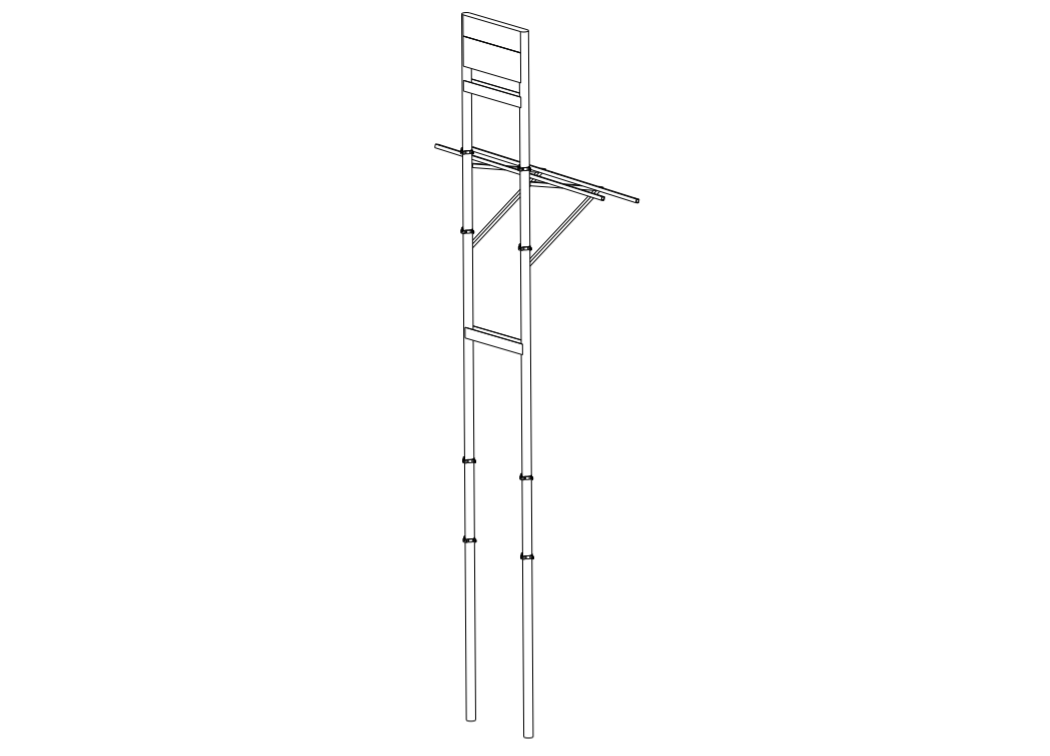
\includegraphics[scale = 0.7]{completa_isometrico.PNG}
            \caption{Estrutura principal: hastes de sustentação.}
            \label{fig:my_label}
        \end{figure}
                
                \item Caixa inferior: Caixa vedada, feita de aço. Responsável pelo armazenamento das baterias. Possui saída para os dutos de fiação.
                
        \begin{figure}[H]
            \centering
            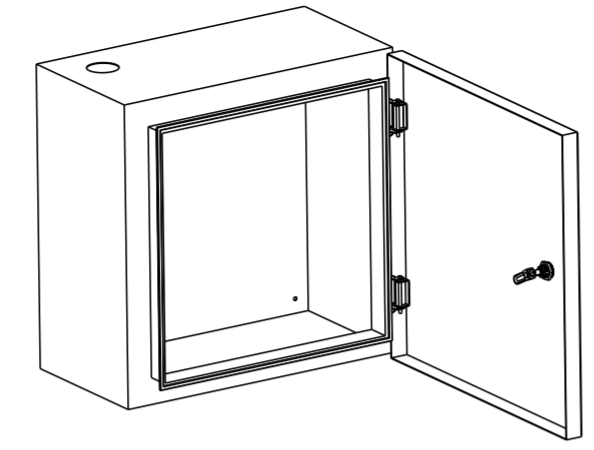
\includegraphics[scale = 0.5]{caixa_1.PNG}
            \caption{Caixa inferior.}
            \label{fig:my_label}
        \end{figure}
        
                \item Caixa Superior: Caixa vedada, feita de aço. Responsável pelo armazenamento dos componentes eletrônicos. Possui o espaço para a alocação do holofote e \emph{cooler}.
                
        \begin{figure}[H]
            \centering
            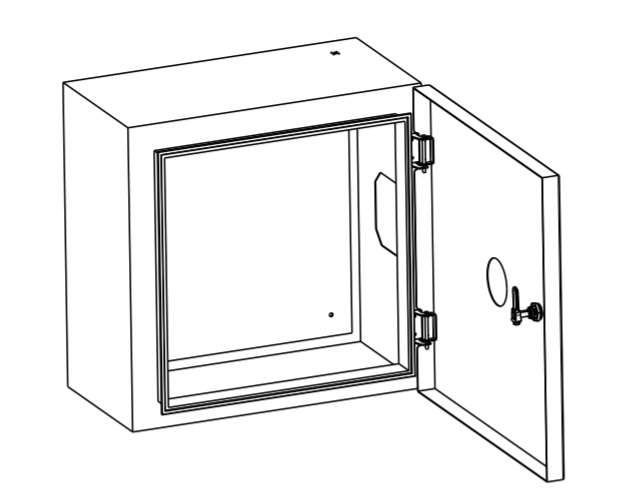
\includegraphics[scale = 0.5]{caixa_2.PNG}
            \caption{Caixa superior.}
            \label{fig:my_label}
        \end{figure}
        
                \item Abraçadeiras metálicas: Abraçadeiras feitas de aço inox. Responsáveis pela fixação das caixas inferior e superior à estrutura principal.
                Parafusos feitos de aço inox.
                
        \begin{figure}[H]
            \centering
            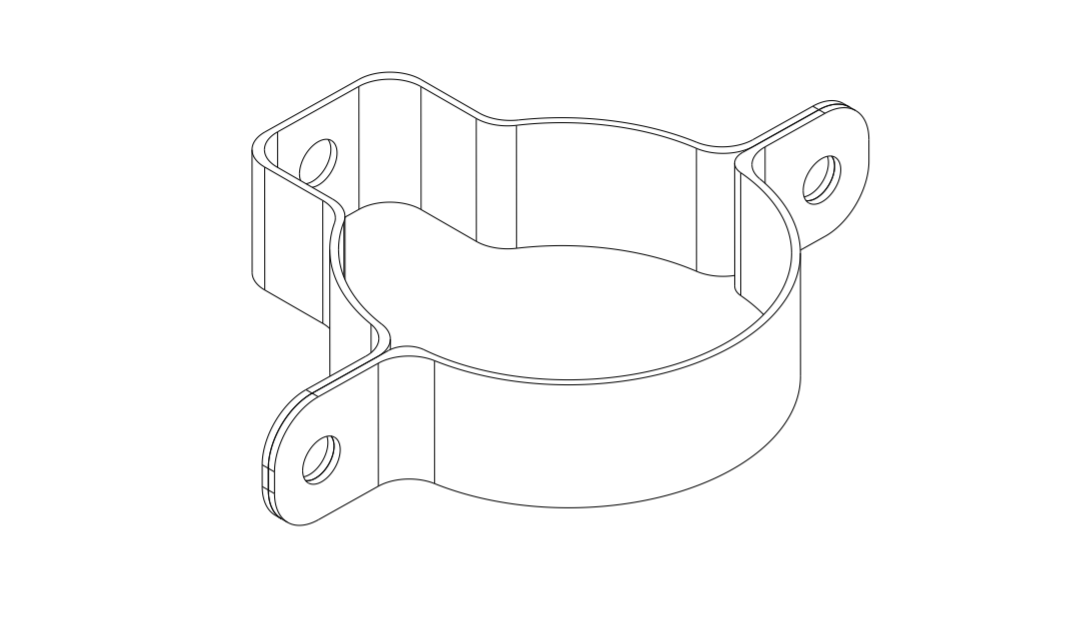
\includegraphics[scale = 0.4]{abracadeira.PNG}
            \caption{Abraçadeira.}
            \label{fig:my_label}
        \end{figure}
         

            \end{enumerate}
             \end{itemize}
        
        \subsubsection{RaDop - Montagem Estrutura}
        
        O passo a passo fornecidos nesse manual de montagem são os passos a serem seguidos na montagem dos módulos. 
        
        Atente-se ao fato de que as caixas serão fixadas à estrutura principal por meio das abraçadeiras metálicas tipo copo e que o encaixe das abraçadeiras são feitas por meio de parafusos. 
        
        \textbf{Nota: os componentes devem ser instalados seguindo o padrão fornecido aqui. O local de instalação e sentido dos mesmos é relevante para a estrutura.}
        
        \begin{figure}[H]
            \centering
            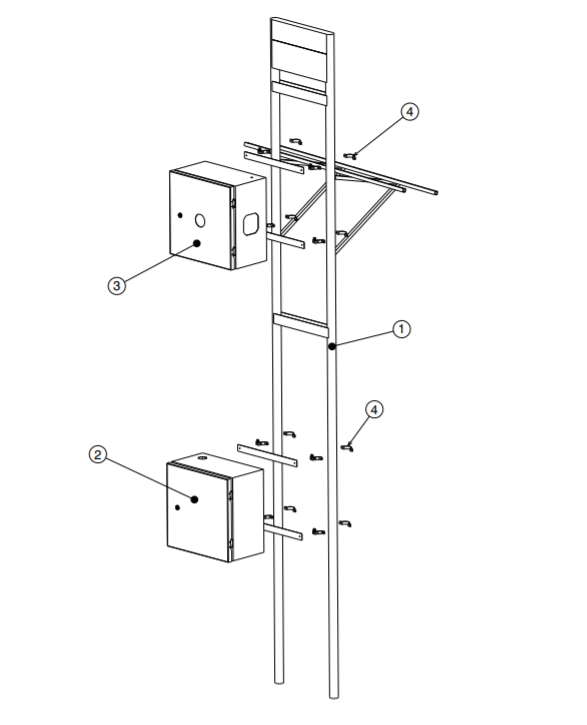
\includegraphics[scale = 0.7]{completa_explodida.PNG}
            \caption{Vista explodida do RaDop com a enumeração das peças para montagem.}
            \label{fig:my_label}
        \end{figure}
        
        
        Instruções:
        \begin{enumerate}
            \item Separe cada módulo e organize-os de forma a identificar cada um pelos números.
            
            \item Separe 4 abraçadeiras metálicas e 8 parafusos para cada caixa.
            
            \item Na caixa inferior (2), fixe as abraçadeiras metálicas com uma distância de 50 mm das arestas. Separe a união e os parafusos para cada abraçadeira.
            
            \item Na caixa superior (3), fixe as abraçadeiras metálicas com uma distância de 50 mm das arestas. Separe a união e os parafusos para cada abraçadeira.
            
            \item Coloque a estrutura principal de forma que ela fique apoiada e que seja possível a instalação dos módulos sem comprometer a integridade física dos mesmos. 
            
            \item Posicione a caixa inferior (2) de acordo com a Figura 6. Certifique-se de que a fechadura está do lado direito. Posicione a caixa de forma que as abraçadeiras metálicas inferiores fique a uma distancia de 1,05 m acima da base da estrutura principal e as abraçadeiras superiores fiquem há 1,45 m acima da base da estrutura principal.
            
            \begin{figure}[H]
            \centering
            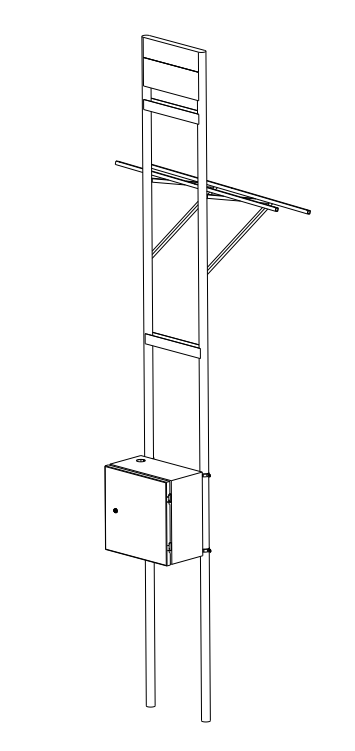
\includegraphics[scale = 0.7]{Caixa1_estrutura.PNG}
            \caption{Estrutura do RaDop com a caixa 1 instalada.}
            \label{fig:my_label}
        \end{figure}
            
            
            \item Coloque a união de cada abraçadeira na caixa 2 e parafuse-as. Certifique de que estão bem parafusadas e que a caixa está bem posicionada e firme.
            
            \item Posicione a caixa superior (3) da mesma forma que foi feita com a caixa (2). Certifique-se que a fechadura está do lado direito. Posicione a caixa para que as abraçadeiras inferiores fiquem há 1,81 m acima da base da estrutura principal e as abraçadeiras superiores fiquem há 2,21m acima da base da estrutura principal.
            
            \item Coloque a união de cada abraçadeira na caixa 3 e parafuse-as. Certifique de que estão bem parafusadas e que a caixa está bem posicionada e firme. Após a instalação da caixa superior (3), a estrutura estará completa.
            
            Após a instalação de todos os módulos, o RaDop deverá estar da seguinte forma:
            
            
            \begin{figure}[H]
                 \centering
                 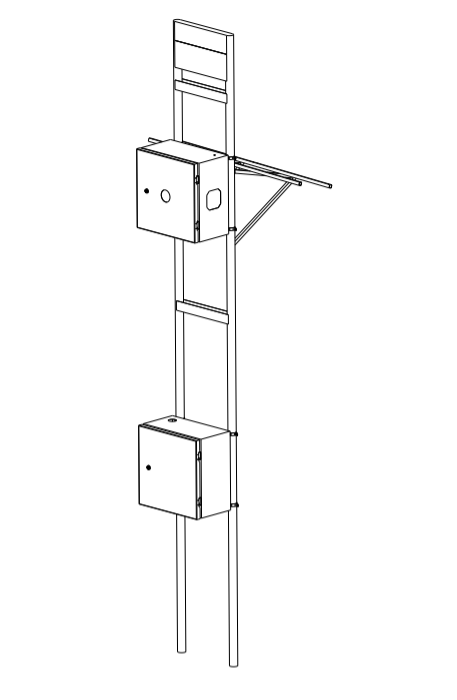
\includegraphics[scale=0.8]{Completa1_isometrica.PNG}
                 \caption{Estrutura após a instalação da caixa 2. Vista isométrica da estrutura completa e montada.}
                 \label{fig:my_label}
             \end{figure}
            
            \item Transporte a estrutura principal com todos os módulos instalados para o local de instalação. 
            Para a fundação, faça 2 buracos de 1 metro de profundidade e com uma distância de 45 cm entre eles (distância entre as hastes da estrutura principal). 
            
            \item Posicione a estrutura principal colocando a fundação das duas hastes nos buracos cavados. Concrete-a no chão. 
            
            \begin{figure}[H]
                 \centering
                 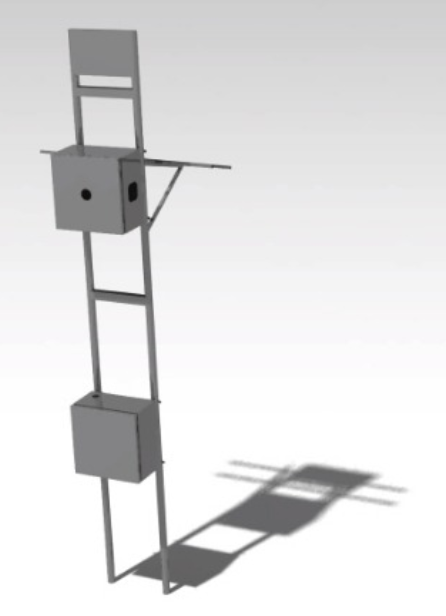
\includegraphics[scale=1]{rende.PNG}
                 \caption{RaDop completo e renderizado.}
                 \label{fig:my_label}
             \end{figure}
            

            
%            \subsubsection{RaDop - Montagem Fiação}
            
%Após a instalação da estrutura completa na fundação, é necessário conectar os fios para poder ligar o sistema elétrico do projeto.

%Existem 3 tipos de cabo no projeto, seguindo o diagrama unifilar:
     
%     \begin{itemize}
%        \item Cabo vermelho: positivo.
%         \item Cabo preto: negativo.
%         \item Cabo verde: aterramento.
%         
%         Dimensão: $2,5mm^2 e 4mm^2$
%     \end{itemize}
     
%A conexão do painel solar é ligada na caixa de bateria. 

%A caixa da bateria tem uma ligação com a caixa de controle.
     
%    \item Utilize o aplicativo para verificar o funcionamento do sistema. 
             
        \end{enumerate}
            
             \subsection{RaDop - Energia}
             
O sistema de alimentação de energia do RaDop é composto por 6 componentes que juntos vão alimentar corretamente o sistema de cargas, para o funcionamento de 3 horas.

             \begin{itemize}
                 \item Componentes:
             \end{itemize}
             \begin{enumerate}
                 
             \item Painéis Fotovoltaicos - 2 unidades de 45Wp;
             
             \item DPS - 1 unidade;
             \item Controlador de Carga - 1 unidade de 12V 30A;
             
             \item Bateria - 2 unidades de 7Ah 12V;
             
             \item Conversores DC/DC - 3 unidades \emph{Step-Down} e 1 \emph{Step-Up};
             
             \item Condutores de $4mm^2$.
             \end{enumerate}
             
              \begin{itemize}
                 \item Função:
             \end{itemize}
             
Os painéis fotovoltaicos são responsáveis pela geração através da incidência solar, sendo necessário o ligamento de dois painéis de 45Wp para o suprimento energético do radar durante 3 horas. Em seguida o dispositivo de proteção contra surtos será responsável por prevenir que descargas atmosféricas danifique o sistema de alimentação de cargas.
             
O controlador de carga vai definir o quanto de tensão e corrente vai ser passado para a alimentação das cargas, essa tensão e corrente será fornecida através do banco de baterias que o sistema terá.
             
Antes da alimentação da carga, a tensão será regulada pelos conversores DC/DC, quando tiver necessidade de elevar ou diminuir a tensão. Por fim, o condutor com a bitola de $2,5 mm^2$  também faz parte dos componentes de energia sendo capazes de suportar a corrente na qual serão submetidos.
             
    \subsubsection{RaDop - Montagem Energia}
             
    Antes de manusear, instalar ou fazer qualquer tipo de manutenção nos painéis solares é ideal ler as instruções e alertas constantes nesse manual. A não observância dessas instruções poderá causar riscos e danos graves para o sistema e para as pessoas. 
             
    Os componentes devem ser instalados conforma dita este manual, a ligação de forma geral e representativa encontrasse no diagrama unifilar.
             
             \begin{enumerate}
                 \item Posicione os painéis no suporte, garantindo firmeza e angulação correta.
              
                 \item	Conecte os painéis em paralelo para garantir que a corrente do sistema seja suprida, os condutores utilizados possuem a seção transversal de $2,5 mm^2$.
                 
                 \item Em seguida conecte a saída dos painéis no controlador de carga.
                 
                  \item Antes da alimentação da carga, as tensões serão reguladas pelos conversores DC/DC, quando necessário diminuir a tensão será utilizado o \emph{Step-Down} e quando necessário aumentar a tensão, será utilizado o \emph{Step-Up}. 
                  
                 \item Após regular a tensão o sistema irá alimentar a carga do RaDop.
                 
                \item A saída do controlador de carga para a alimentação das cargas será ligado inicialmente no disjuntor geral que em paralelo será ligado no dispositivo de proteção contra surtos (DPS) e sua saída aterrada no aterramento do sistema elétrico.
                 
                 \item A saída dos disjuntores irá alimentar as cargas com o objetivo de impedir surtos em caso de sobrecarga ou de qualquer outro surto que danifique o circuito de alimentação das cargas.
                
                 \item As baterias devem ser ligadas em paralelo entre si, para garantir o fornecimento correto de corrente ao sistema e ligadas no controlador de carga.
                 
                 \item As baterias possuem um suporte específico, logo devem ser posicionadas nele.
                 
                 \item a fiação das baterias devem ser posicionadas no eletroduto feito pra isso. Os condutores utilizados foram de seção $ 4mm^2$.
                 
                 \item a utilização do fusível antes de alimentar a USRP é importante pela sensibilidade do equipamento.

             \end{enumerate}

\subsection{RaDop -Eletrônica}
O sistema eletrônico do RaDop é composto por:

\begin{itemize}
         \item Componentes:
         \end{itemize}
         \begin{enumerate}
    \item \emph{Raspberry} Pi 3 - 1 unidade; 
    \item USRP NI2901 - 1 unidade;
    \item Câmera - 1 unidade;
    \item \emph{Switch} - 1 unidade;
    \item Holofote - 1 unidade;
    \item \emph{Cooler} - 1 unidade;
    \item Relé 5V 2 canais - 1 Unidade;
    \item Módulo NRF24L01 com antena externa - 1 unidade;
    \item Cabo coaxial RF - 2 unidades;
    \item Antenas - 2 unidades.
    \end{enumerate}

\begin{itemize}
       \item Função:
\end{itemize}

A \emph{Raspberry} Pi 3 é responsável por fazer a comunicação entre os módulos e o controle de funcionalidade de cada um deles. O rádio definido por software USRP NI2901 é responsável por fazer a conversão AD dos dados de transmissão com amplificação e na recepção convertendo novamente os dados.  O \emph{switch} é responsável pela rede local que comunica a câmera com a \emph{Raspberry}, além de também fazer a comunicação com o servidor. A câmera é responsável por fazer a captura da parte traseira do carro quando este cometer uma infração. O holofote é uma sinalização luminosa que visa alertar os condutores para riscos de provável acidente, o \emph{cooler} para que a caixa não esquente muito, o módulo NRF24L01 é responsável pela comunicação entre os totens, as antenas para propagação da onde eletromagnética de envio e recepção, e os cabos coaxiais para conectar as antenas ao USRP.

  \subsubsection{RaDop - Montagem Eletrônica}
  Após serem feitas as montagem e testes com o sistema de alimentação descrito na \emph{montagem energia}, deve-se inicializar a montagem e colocação dos componentes eletrônicos. Os componentes devem ser conectados conforme este manual, e com o máximo de cuidado para que os cabos não fiquem dobrados.
  
  \begin{enumerate} 
  \item Conecte os cabos coaxiais entre as antenas e o USRP. Lembre-se de conectar um cabo em Tx e o outro em Rx no mesmo canal.  
  \item  Conecte o cabo USB entre o USRP e a Raspberry Pi 3 
  \item Conecte o cabo de rede externo com conector RJ45 na entrada azul do \emph{switch}
  \item Conecte o cabo de rede com conector RJ45 saindo da entrada amarela do \emph{switch} para o conector \emph{ethernet} da Raspberry Pi 3. 
  \item Conecte o cabo de rede com conector RJ45 saindo da entrada amarela do \emph{switch} para o conector \emph{ethernet} na câmera.
  \item Conecte os \emph{jumpers} entre a Raspberry Pi 3 e o módulo NRF24, como descrito na Tabela \ref{nrf}.
  \item Conecte os \emph{jumpers} entre a Raspberry Pi 3 e o módulo relé, como descrito na Tabela \ref{mon}.
  \item Conecte a alimentação do \emph{cooler} no canal 1 do relé de modo normalmente fechado.
  \item Conecte a alimentação do holofote no canal 2 do relé de modo normalmente fechado. 
  \item Através do conector USB disponível no controlador de carga, conecte no microUSB da Raspberry Pi 3 para alimentação.  
  \item Conecte o cabo de alimentação da Câmera e do USRP.
  \end{enumerate}


\begin{table}[H]
\centering
\caption{Conexão entre a Raspberry Pi 3 e o módulo NRF24L01}
\begin{tabular}{cc}
Raspberry Pi 3 & NRF24L01 \\
Pin 15         & CE       \\
Pin 17         & VCC      \\
Pin 19         & MOSI     \\
Pin 21         & MISO     \\
Pin 23         & SCK      \\
Pin 25         & GND      \\
Pin 24         & CSN     
\end{tabular}
\label{nrf}
\end{table}

\begin{table}[H]
\centering
\caption{Conexão entre a Raspberry Pi 3 e o módulo relé}
\begin{tabular}{cc}
Raspberry Pi 3 & Relé \\
Pin 04         & VCC  \\
Pin 08         & CH1  \\
Pin 10         & CH2  \\
Pin 06         & GND 
\end{tabular}

\label{mon}
\end{table}


\subsubsection{RaDop - Funcionamento Eletrônica}
Para este procedimento, conecte um computador externo na rede local para acesso remoto através de ssh ou vnc para controle da Raspberry Pi 3.
  \begin{enumerate} 
\item Conectado na mesma rede local, abra o \emph{Windows Explorer} e acesse o seguinte endereço http://10.0.0.100 para acesso às configurações da câmera.
\item Com usuário \emph{admin} crie uma senha pessoal para acesso restrito à ela e configure.
\item No ambiente \emph{Raspbian} na Raspberry Pi 3, entre no terminal e dê o comando controle.py.
\end{enumerate}

\subsection{RaDop - Software}

Todos os sistemas de software do Radar foram feitos com uma boa interface e de fácil usabilidade para que os usuários não tivessem problemas com as funcionalidades dos sistemas. 

\subsubsection{Dashboard}

A tela principal, como mostra a Figura \ref{home}, do radar é onde contém boa parte do \textit{Business intelligence (BI)} e também não precisa de acesso para conseguir visualizar estes dados.


  \begin{figure}[H]
     \centering
     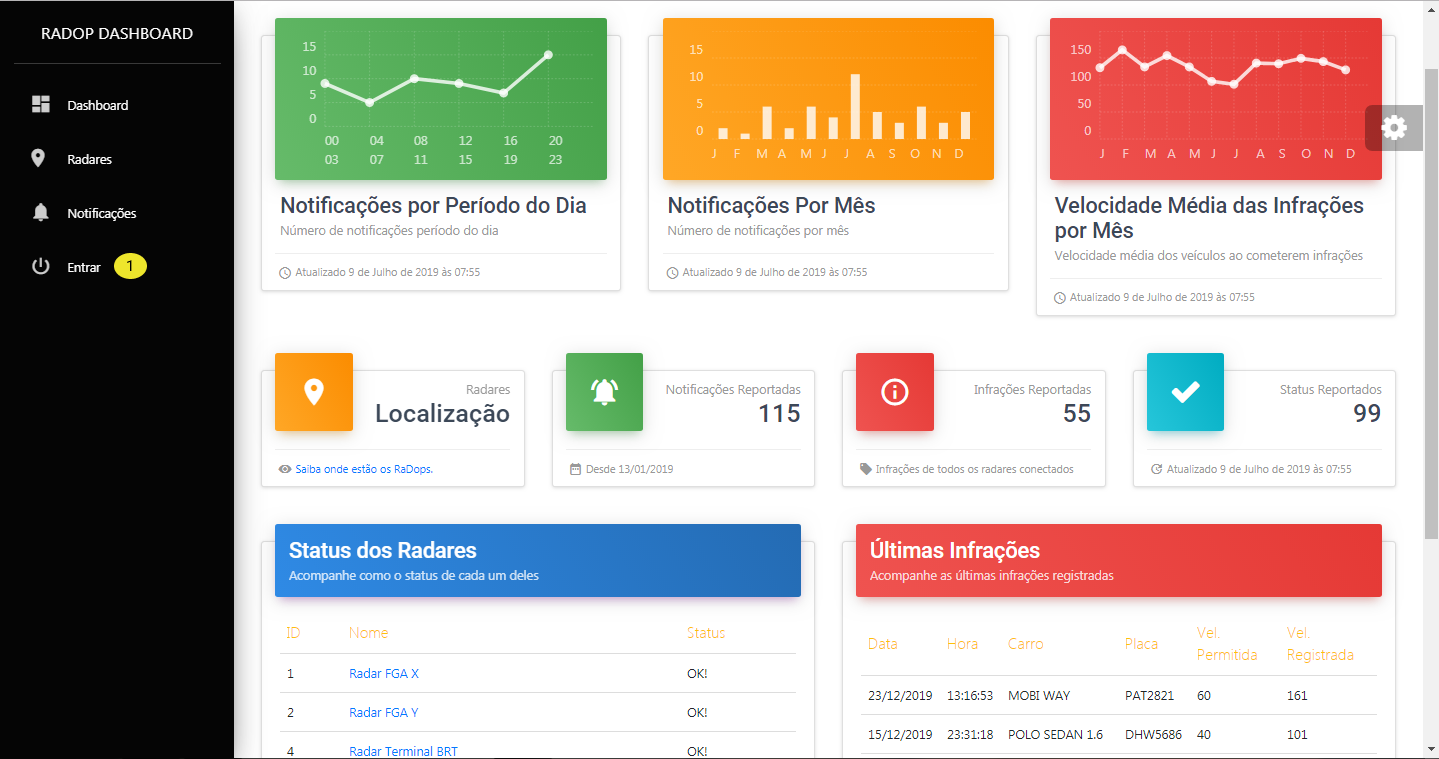
\includegraphics[scale=0.25]{home.png}
     \caption{Página inicial do \textit{Dashboard}.}
     \label{home}
 \end{figure}

Para acessar as outras informações do radar é preciso realizar o \textit{login} na página login (1), mostrada na Figura \ref{login}. Lembrando que apenas o mantenedor e o administrador do site terão acesso à essas áreas. 

  \begin{figure}[H]
     \centering
     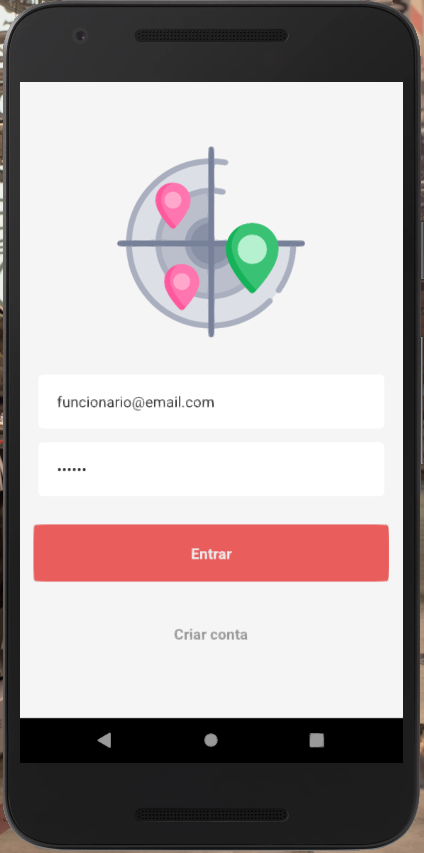
\includegraphics[scale=0.25]{login.PNG}
     \caption{Página de Login do \textit{Dashboard}.}
     \label{login}
 \end{figure}
 
 Após realizar o \textit{login}, o usuário será capaz de acessar a página, mostrada na Figura \ref{home_2} com os radares instalados (2) e com as notificações (3).
 
   \begin{figure}[H]
     \centering
     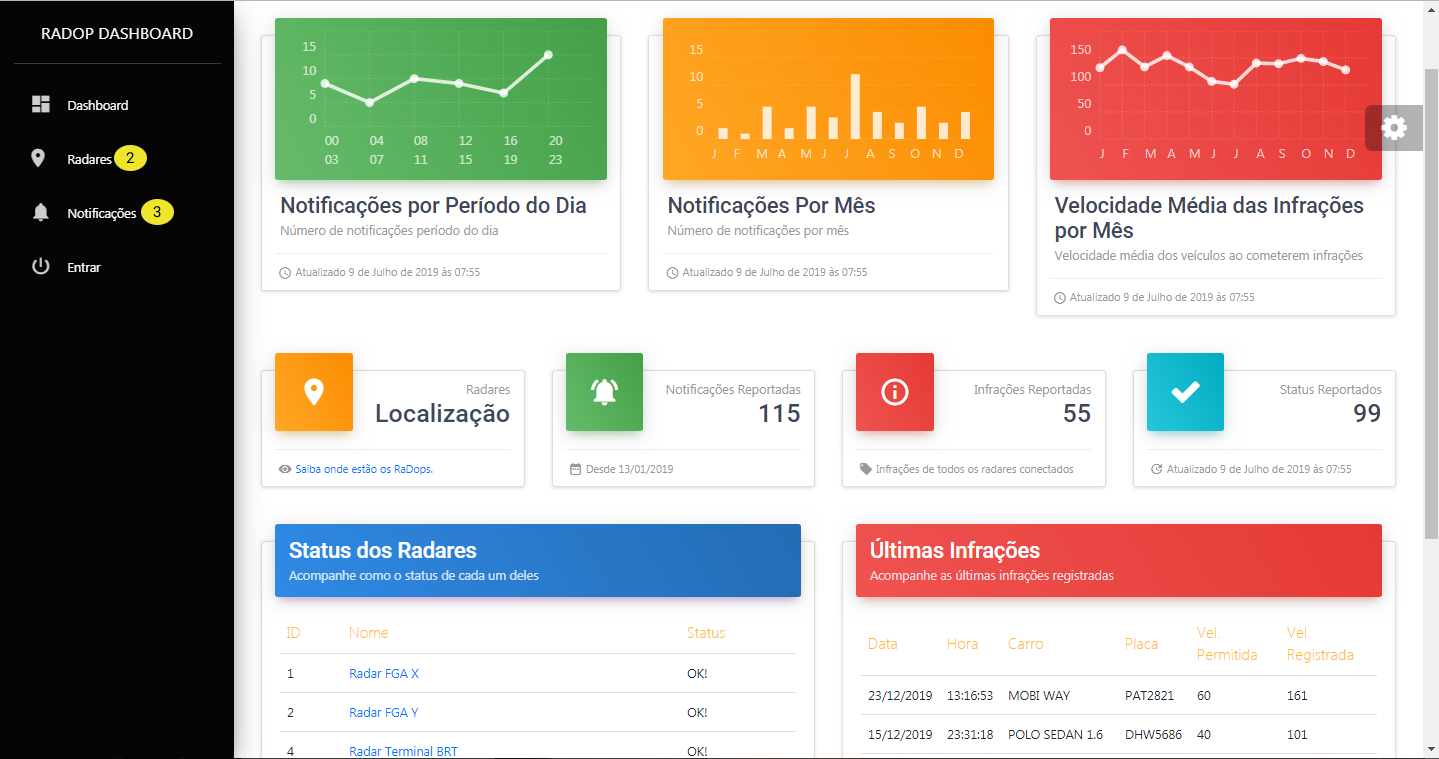
\includegraphics[scale=0.25]{home_2.png}
     \caption{Página inicial do \textit{Dashboard}.}
     \label{home_2}
 \end{figure}

A Figura \ref{radares} mostra todos os radares que estão instalados e o mantenedor terá acesso.

   \begin{figure}[H]
     \centering
     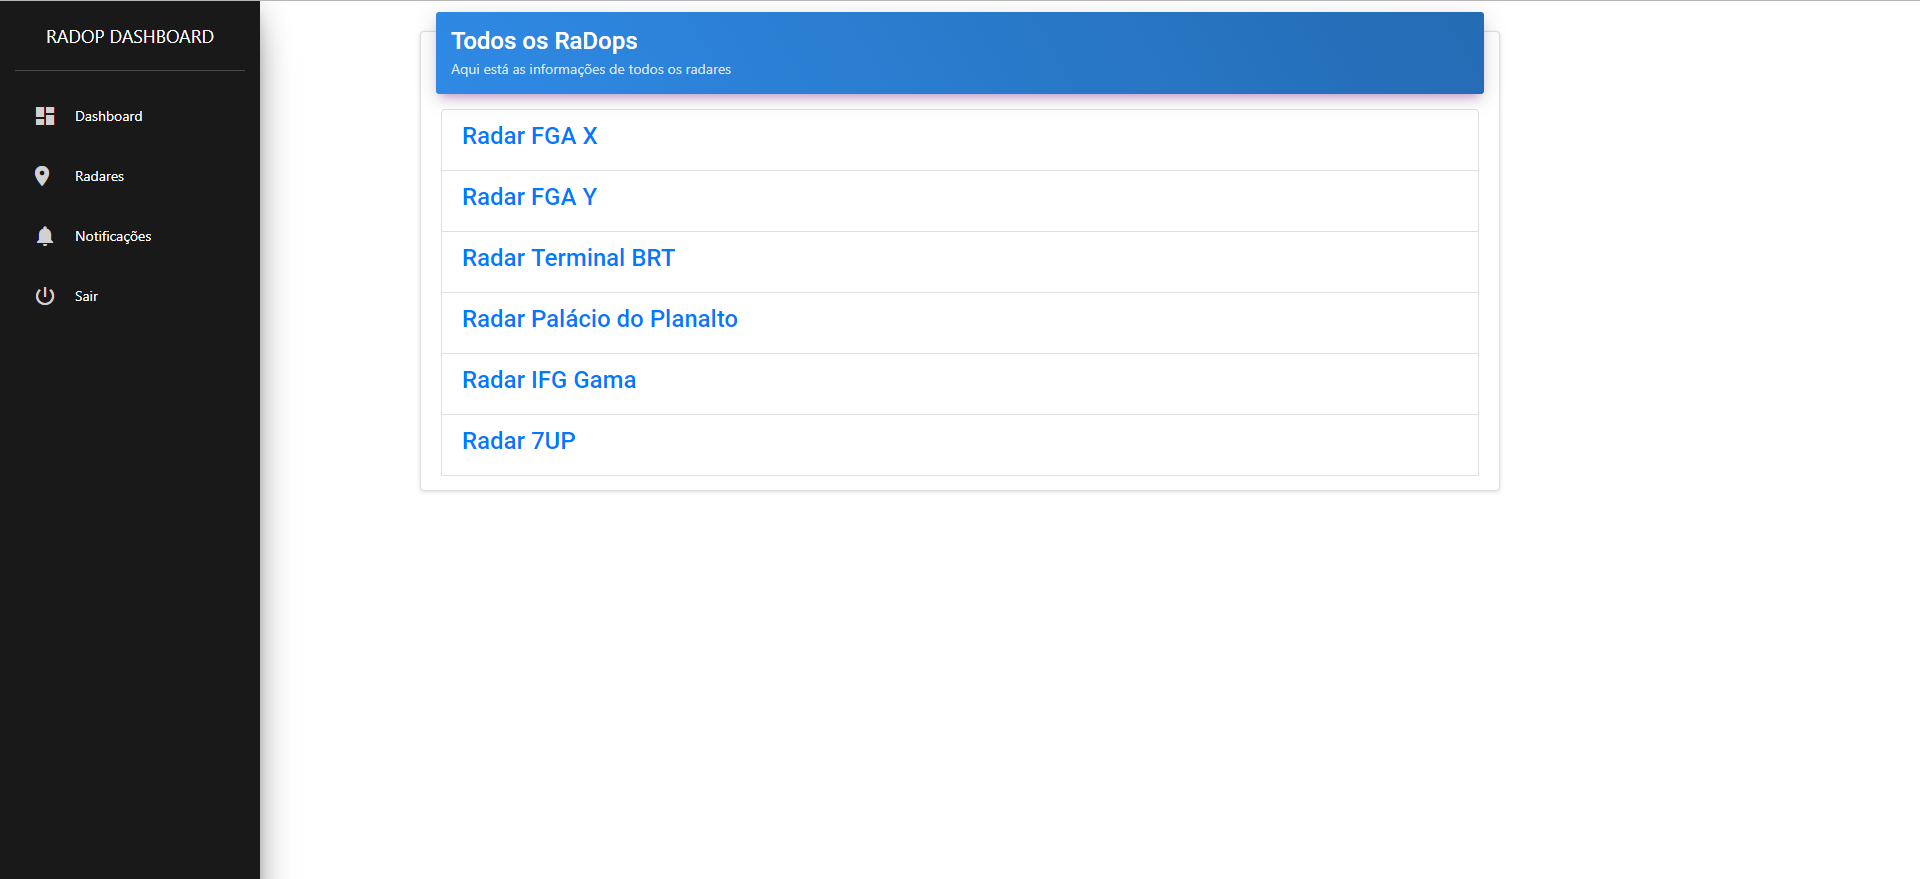
\includegraphics[scale=0.25]{lista_radares.PNG}
     \caption{Página com a lista de todos os radares que estão instalados.}
     \label{radares}
 \end{figure}
 
 Ao acessar algum dos radares listados, o usuário será redirecionado para a página, mostrada na Figura \ref{radar_detail}, com as informações do radar selecionado.
 
    \begin{figure}[H]
     \centering
     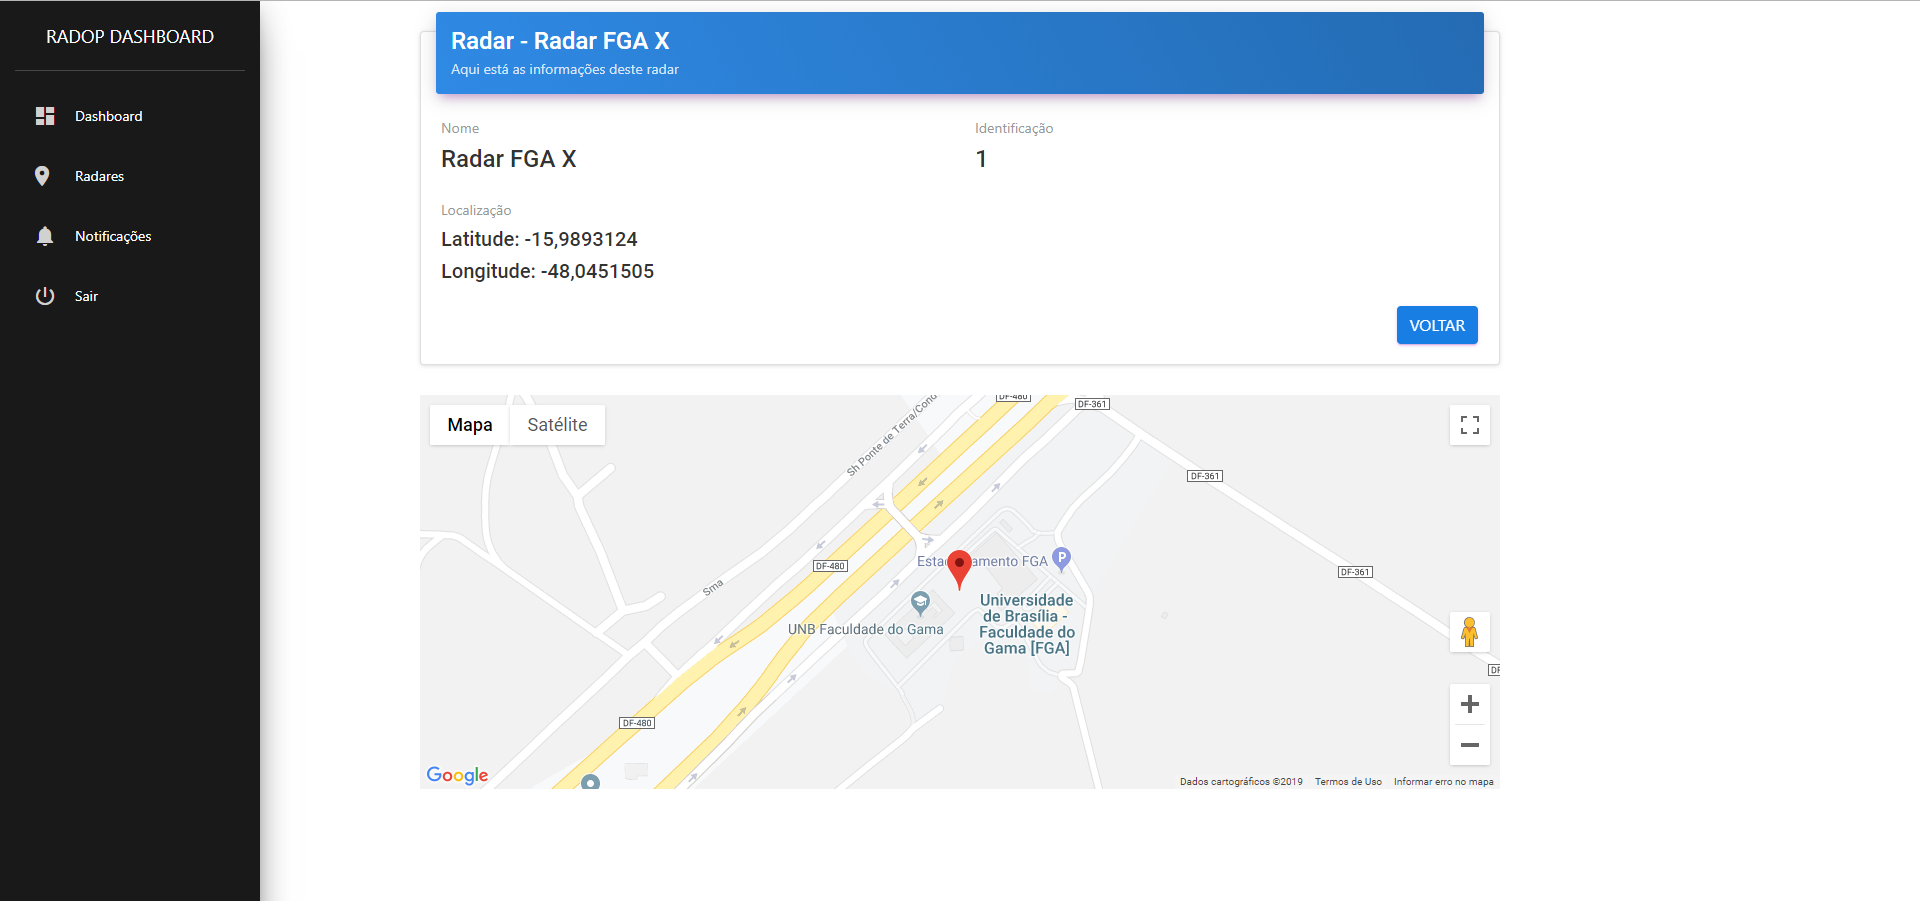
\includegraphics[scale=0.25]{radar_detail.PNG}
     \caption{Página com as informações do radar.}
     \label{radar_detail}
 \end{figure}

Caso o usuário opte por acessar a página com as notificações, ele será redirecionado para uma outra página, mostrada na Figura \ref{lista_notificacao}, com a lista com as notificações de infrações e de possibilidade acidente.

    \begin{figure}[H]
     \centering
     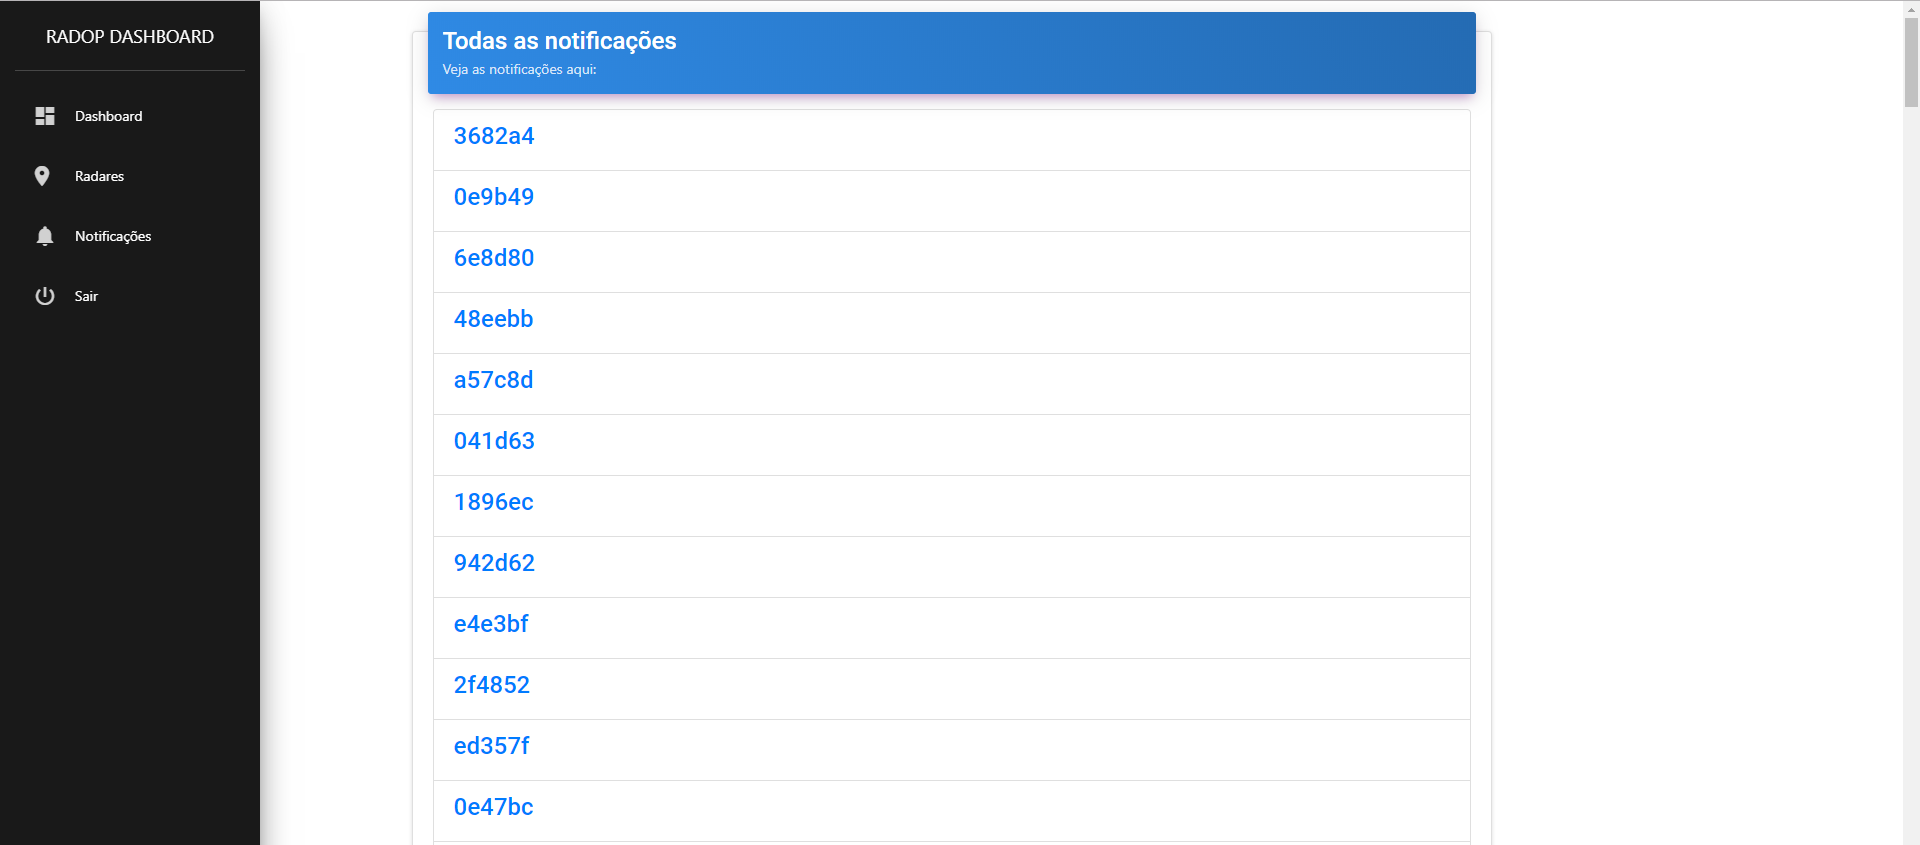
\includegraphics[scale=0.25]{lista_notificacao.PNG}
     \caption{Página com a lista de todos as notificação, tanto de infração, quanto de possibilidade de acidente.}
     \label{lista_notificacao}
 \end{figure}
 
 A Figura \ref{notificacao_detail} mostra que ao acessar alguma das notificações, o usuário terá acesso a todas informações a respeito da notificação e do também do carro notificado. 
 
     \begin{figure}[H]
     \centering
     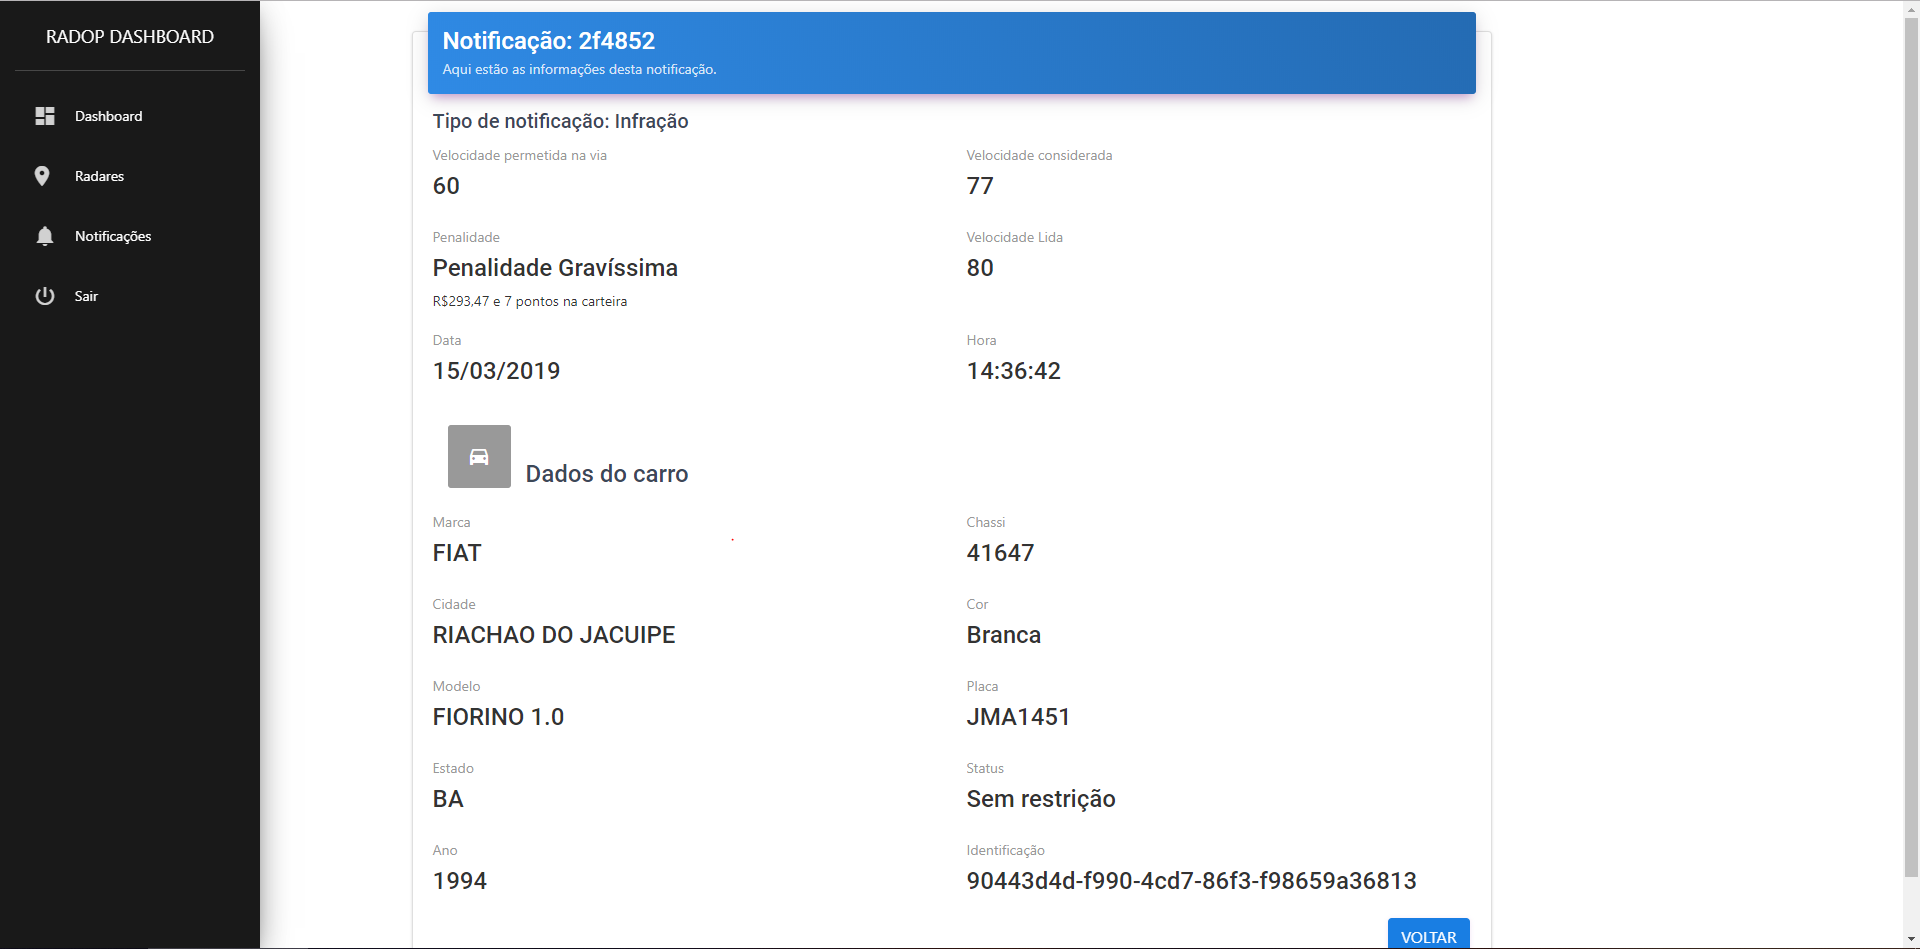
\includegraphics[scale=0.25]{notificacao_detail.PNG}
     \caption{Página com as informações das notificações e do carro notificado.}
     \label{notificacao_detail}
 \end{figure}
 
 

\subsubsection{Aplicativo RaDop}

A tela inicial, como mostra a Figura \ref{fig:app-login}, o usuário é automaticamente direcionado para a tela de autenticação. Nesta tela ele deverá preencher o campo de endereço de e-mail e o campo senha, para que seja enviado ao servidor a solicitação de \textit{login}. Caso haja algum campo errado uma mensagem aparecerá, se não, o usuário será redirecionado para a próxima tela.\footnote{Nesta versão da aplicação é possível criar novas contas, caso o usuário não tenha, mas em próximas versões da aplicação apenas administradores poderão criar novas contas.} 

    \begin{figure}[H]
        \centering
        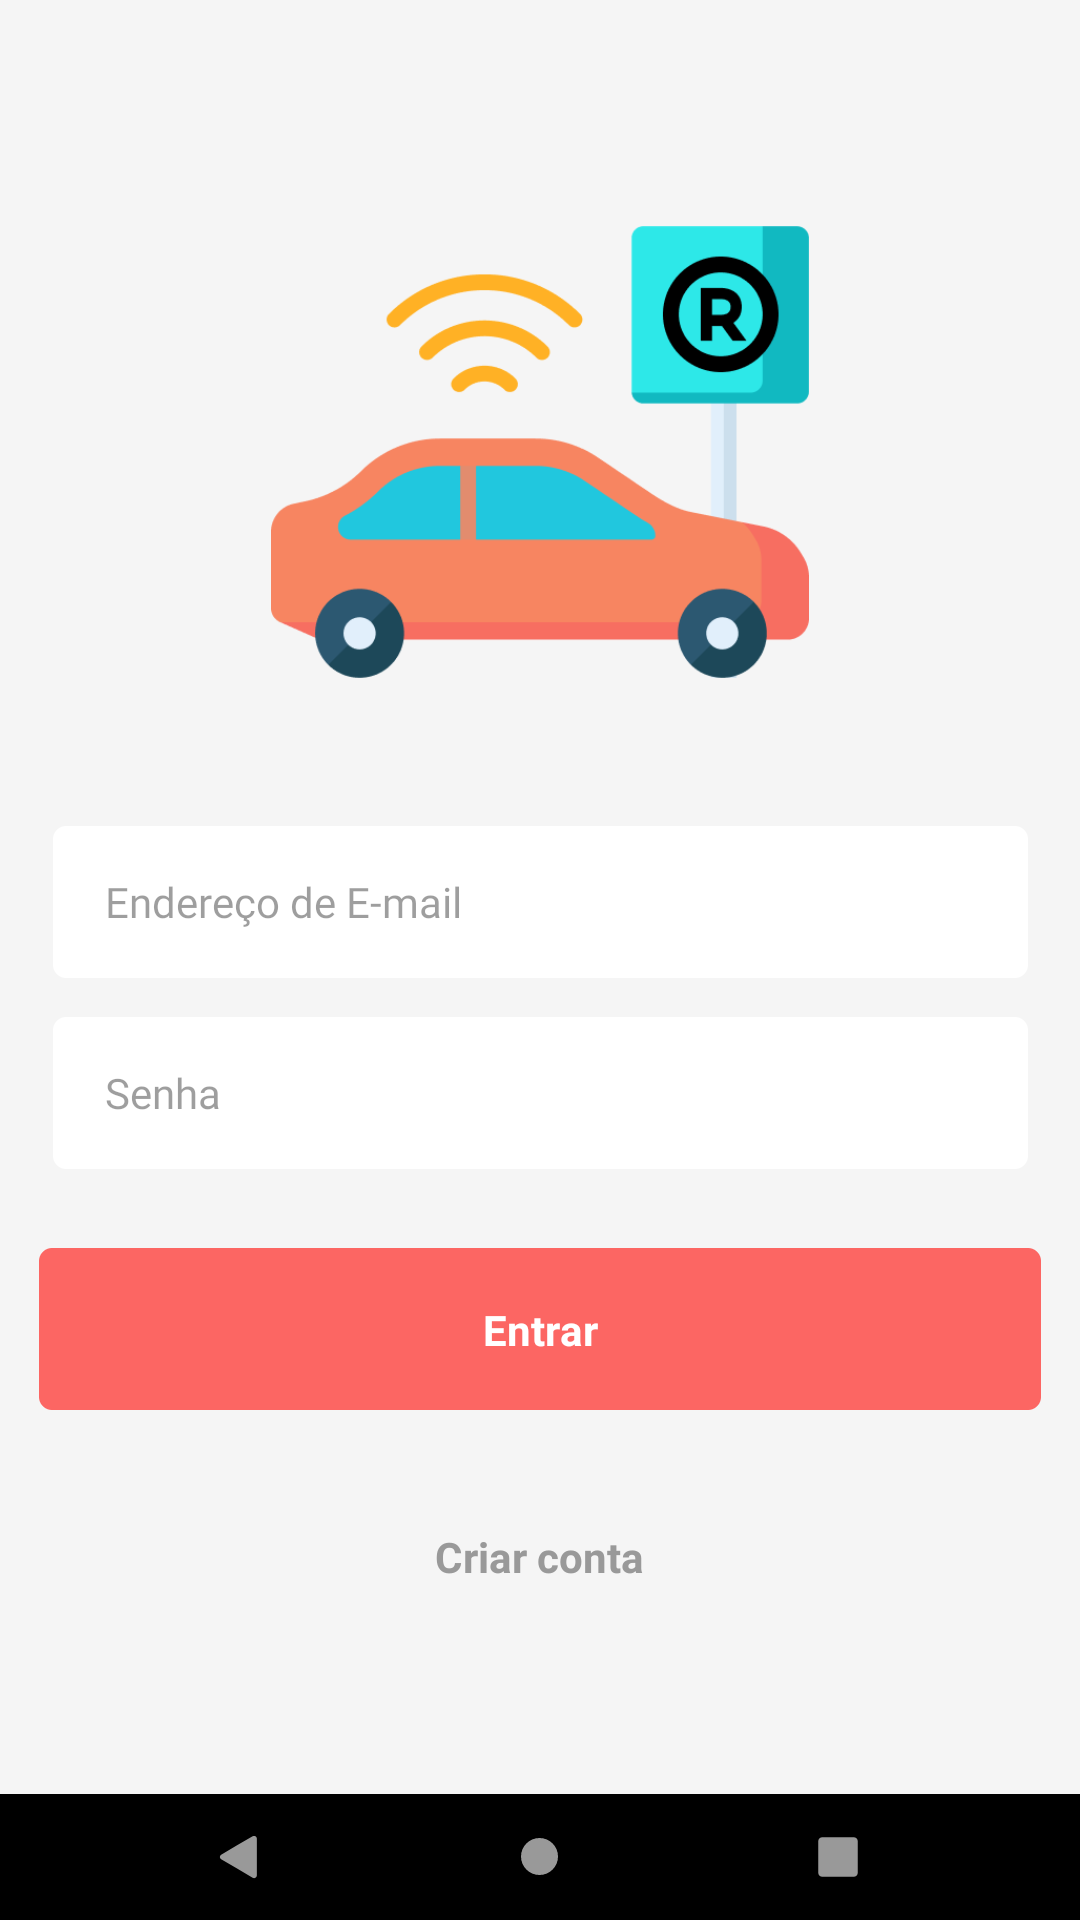
\includegraphics[scale=0.15]{log-manual.png}
        \caption{Tela de autenticação do usuário mantenedor do RaDop.}
        \label{fig:app-login}
    \end{figure}

Com a sessão iniciada na aplicação o usuário será apresentado ao mapa identificando todos os radares presentes à um raio de 15Km (quilômetros) da sua posição atual, conforme é possível ver na Figura \ref{fig:app-inicial}. Os radares estão dispostos em ícones quadrados com a coloração vermelha e são identificados pelo identificador do radar e o nome do radar (\textit{id: nome}). Nesta tela há três opções. Ao clicar no nome do radar o usuário será direcionado para a tela que mostra os estados do radar, que pode ser visto na Figura \ref{fig:app-status}. Ao clicar na opção (1) o usuário indicará ao sistema que deseja ver as manutenções já registradas de um radar, ao clicar na opção (2), indicará que deseja registrar uma nova manutenção.

    \begin{figure}[H]
        \centering
        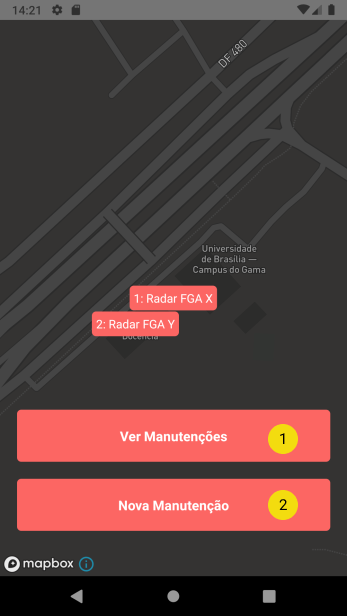
\includegraphics[scale=0.45]{inicial-opcao.png}
        \caption{Tela inicial com as opções as três opções de funcionalidade.}
        \label{fig:app-inicial}
    \end{figure}
    
Com a opção deseja selecionada o sistema pedirá que o usuário selecione um radar para realizar a operação desejada. Basta ao usuário selecionar o radar pressionando a caixa vermelha que envolve o nome e o identificador do radar. Conforme o exemplo abaixo na imagem \ref{fig:app-selecione}.
    
    \begin{figure}[H]
        \centering
        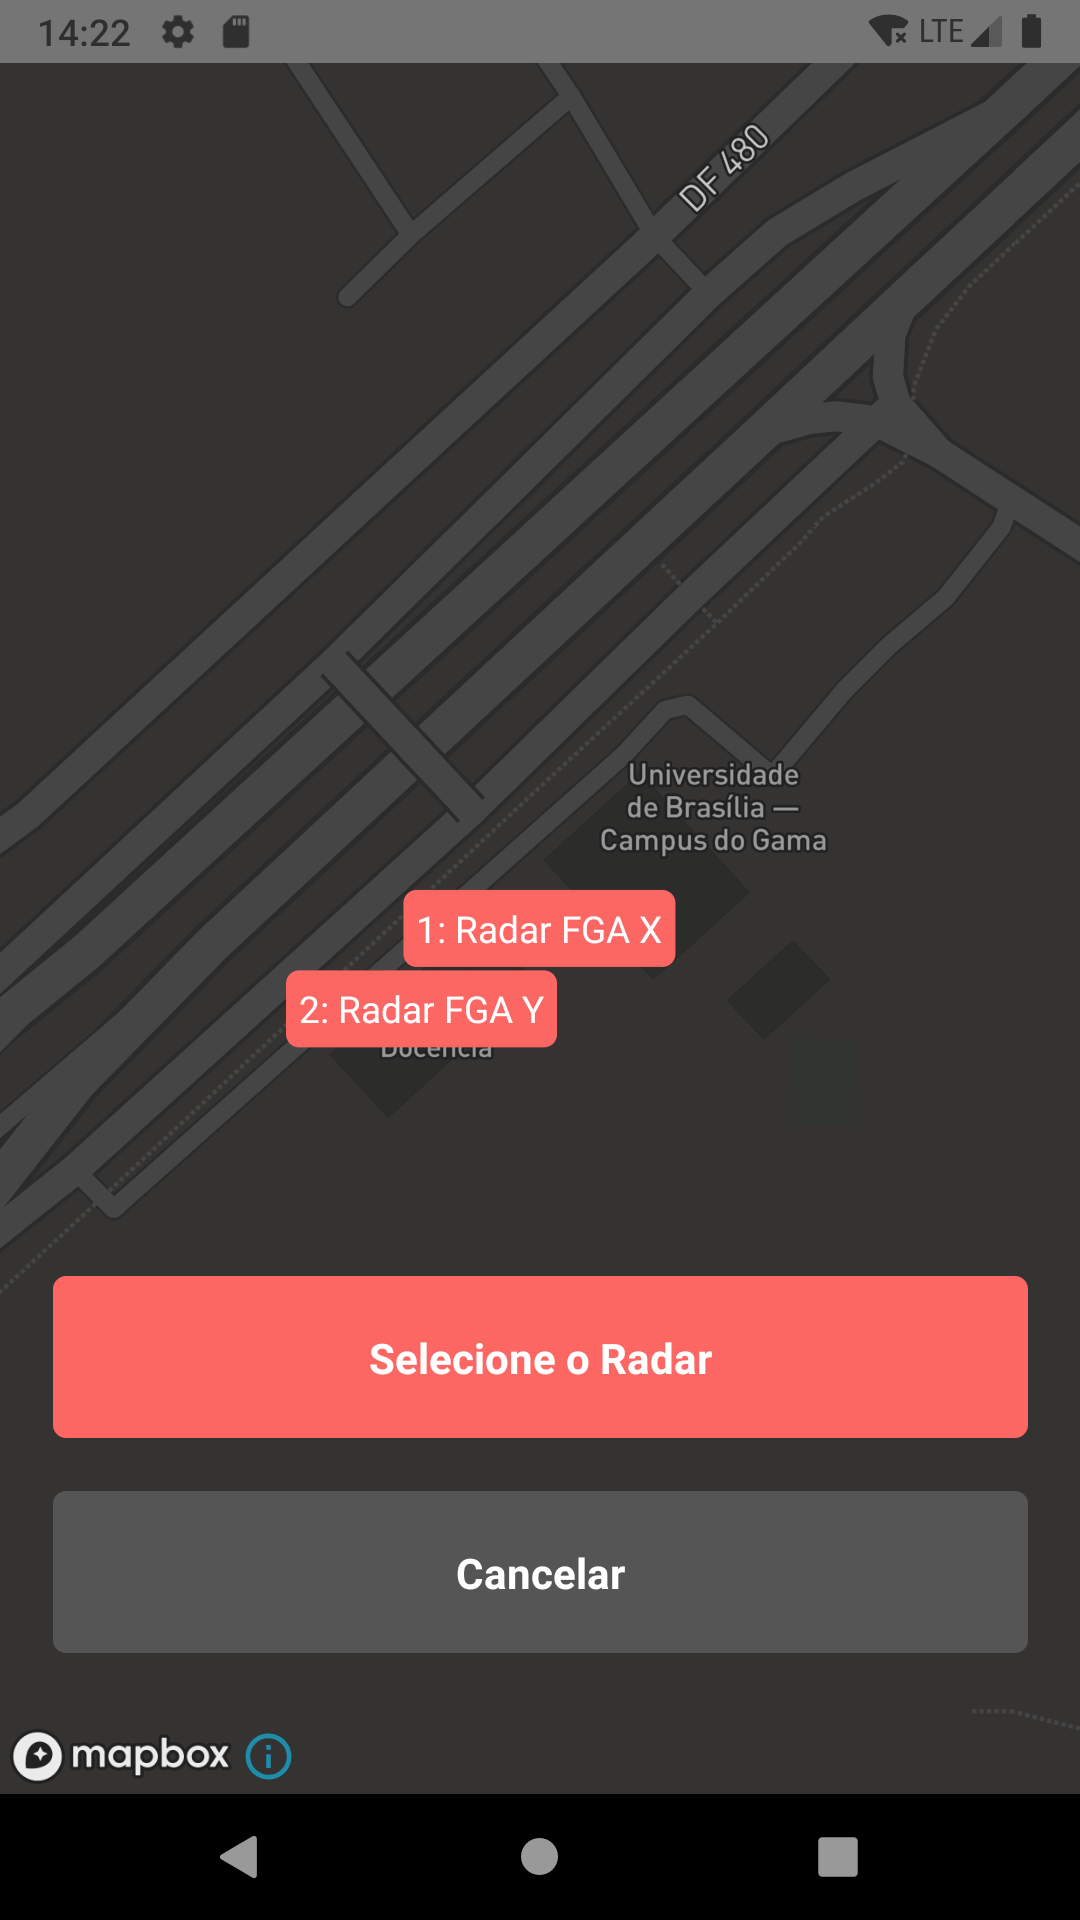
\includegraphics[scale=0.15]{selecione.png}
        \caption{Tela de seleção do radar.}
        \label{fig:app-selecione}
    \end{figure}

Assim que o radar desejado for selecionado o sistema apresentará a mensagem "\textit{Selecionado}" logo após o nome do radar. Agora basta apertar o botão inferior "Selecione o Radar" para confirmar ao sistema a escolha, conforme ilustrado na Figura \ref{fig:app-selecionado}. Caso o usuário deseje, a operação pode ser cancelada bastando pressionar "Cancelar" a qualquer momento.

    \begin{figure}[H]
        \centering
        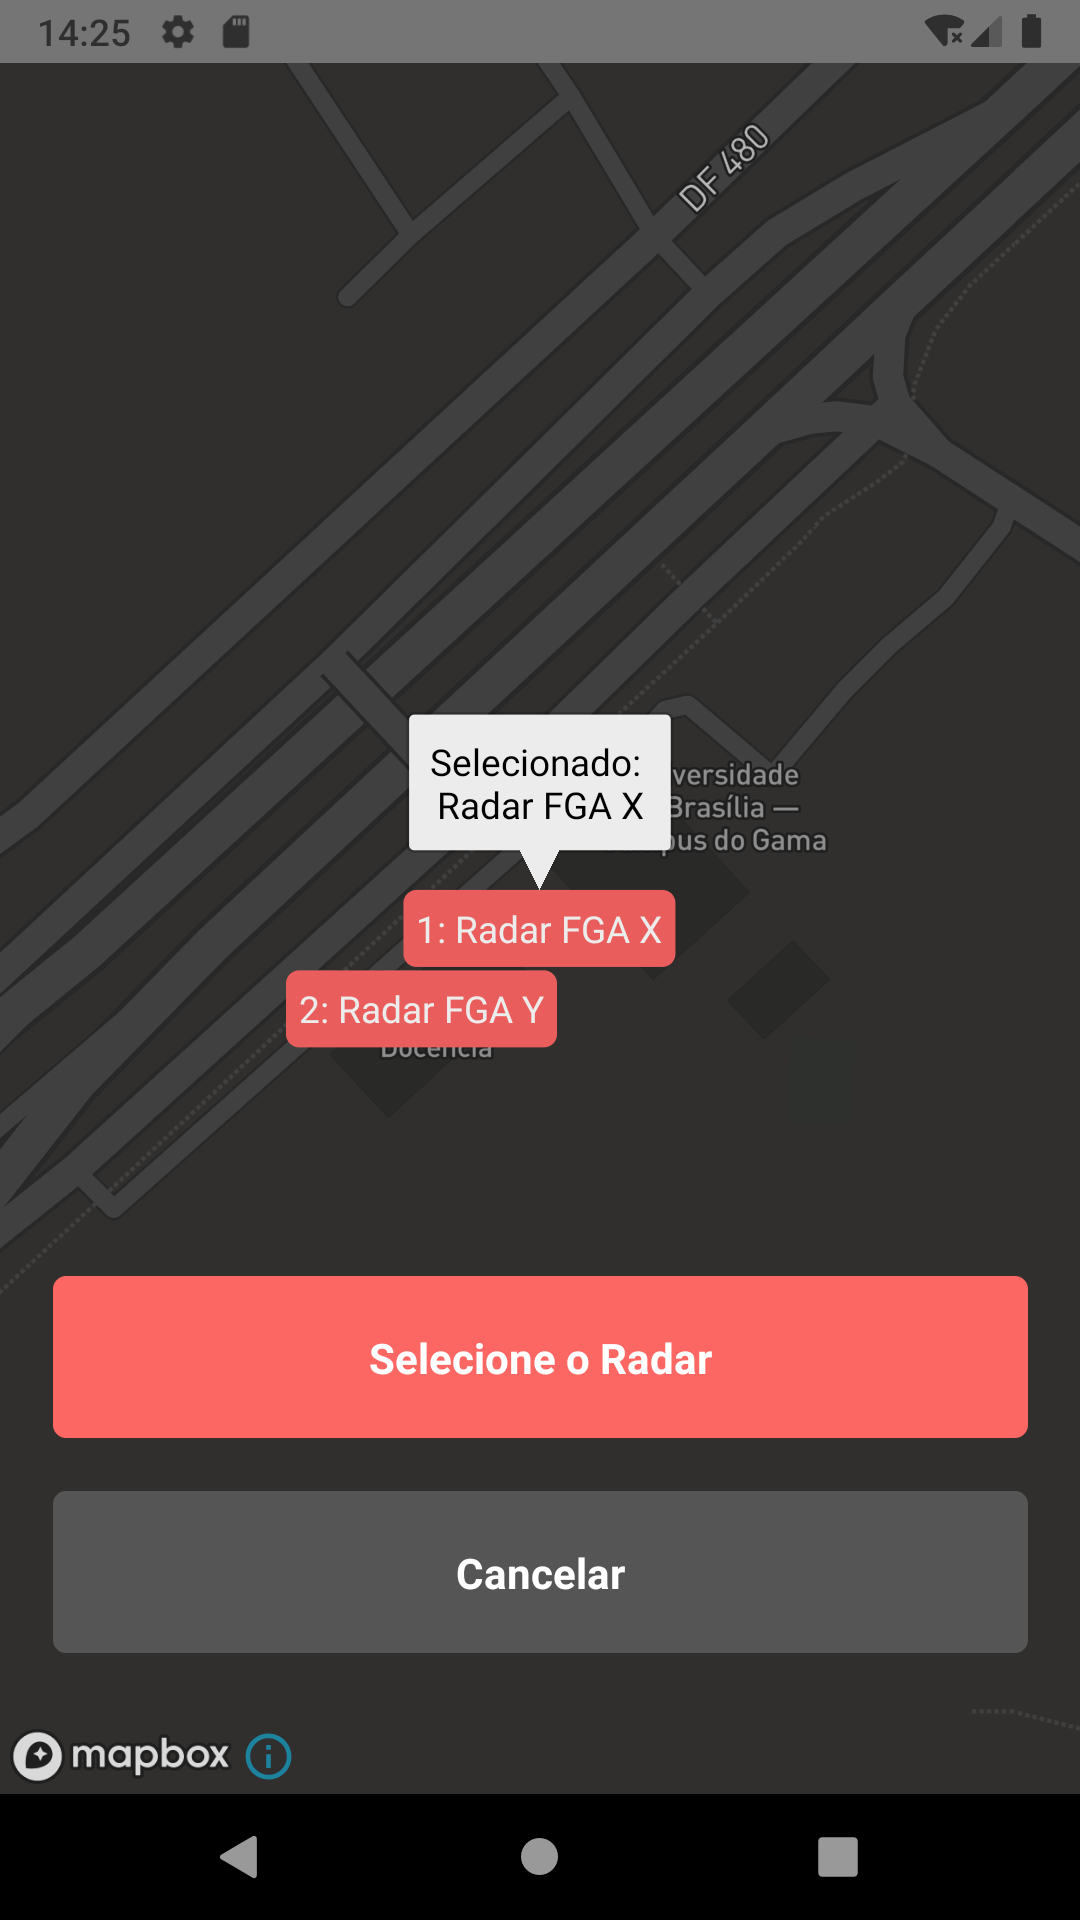
\includegraphics[scale=0.15]{selecionado.png}
        \caption{Tela com o radar selecionado em destaque.}
        \label{fig:app-selecionado}
    \end{figure}

Caso a opção escolhida tenha sido a (1) o usuário será apresentado com a lista das manutenções registradas para o radar. Vide Figura \ref{fig:app-manutencoes}. Após visualizar as manutenções o usuário pode apertar o botão "Fechar" para retornar a tela principal.

    \begin{figure}[H]
        \centering
        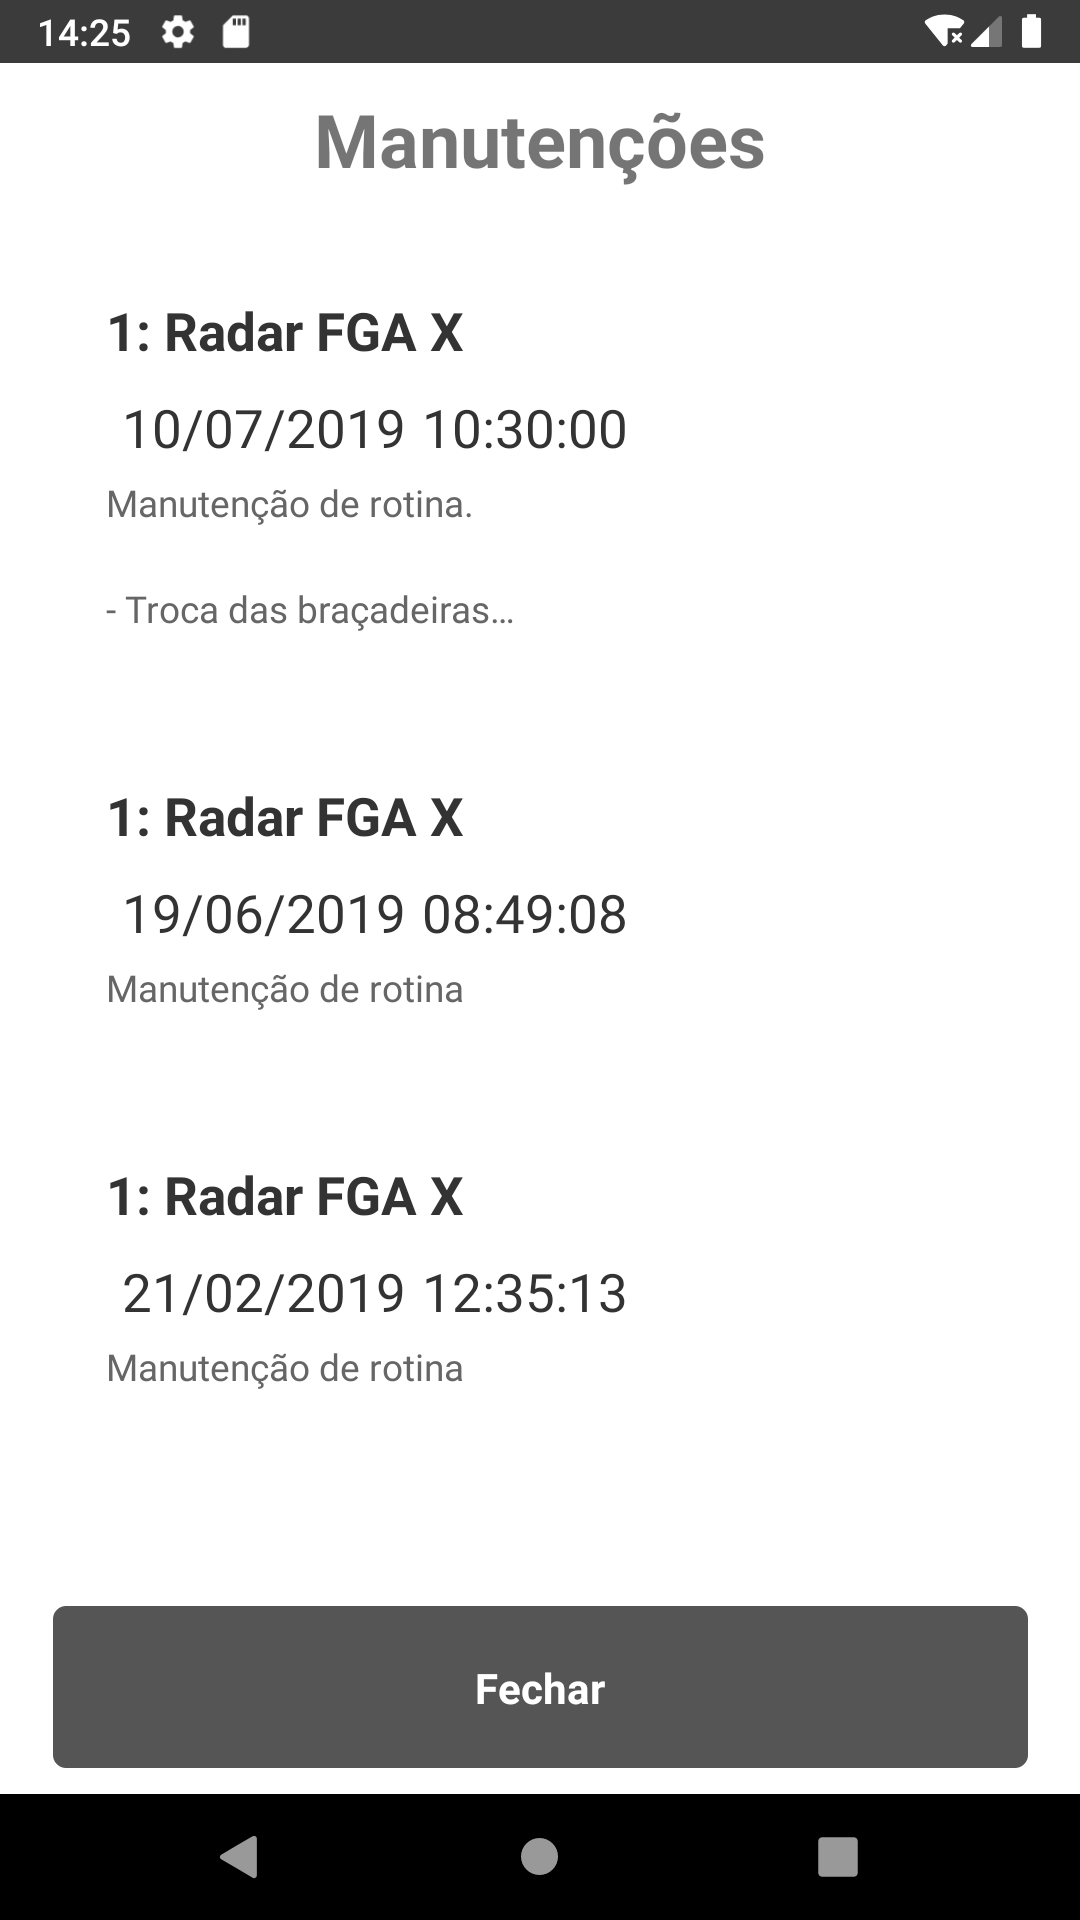
\includegraphics[scale=0.15]{manutencoes.png}
        \caption{Tela com as manutenções feitas no radar selecionado.}
        \label{fig:app-manutencoes}
    \end{figure}

Caso a opção escolhida tenha sido a (2) o usuário será apresentado com o formulário de registro de uma nova informação. Os campos de data e hora apresentarão caixas de seleção para facilitar o registro das informações, e no campo razão o usuário poderá discorrer um texto da razão da manutenção, assim como o que foi executado na manutenção. Vide Figura \ref{fig:app-manutencao}. Caso o usuário queira, o registro da manutenção pode ser cancelado a qualquer momento, se não, basta clicar em salvar para finalizar o registro.
    
    \begin{figure}[H]
        \centering
        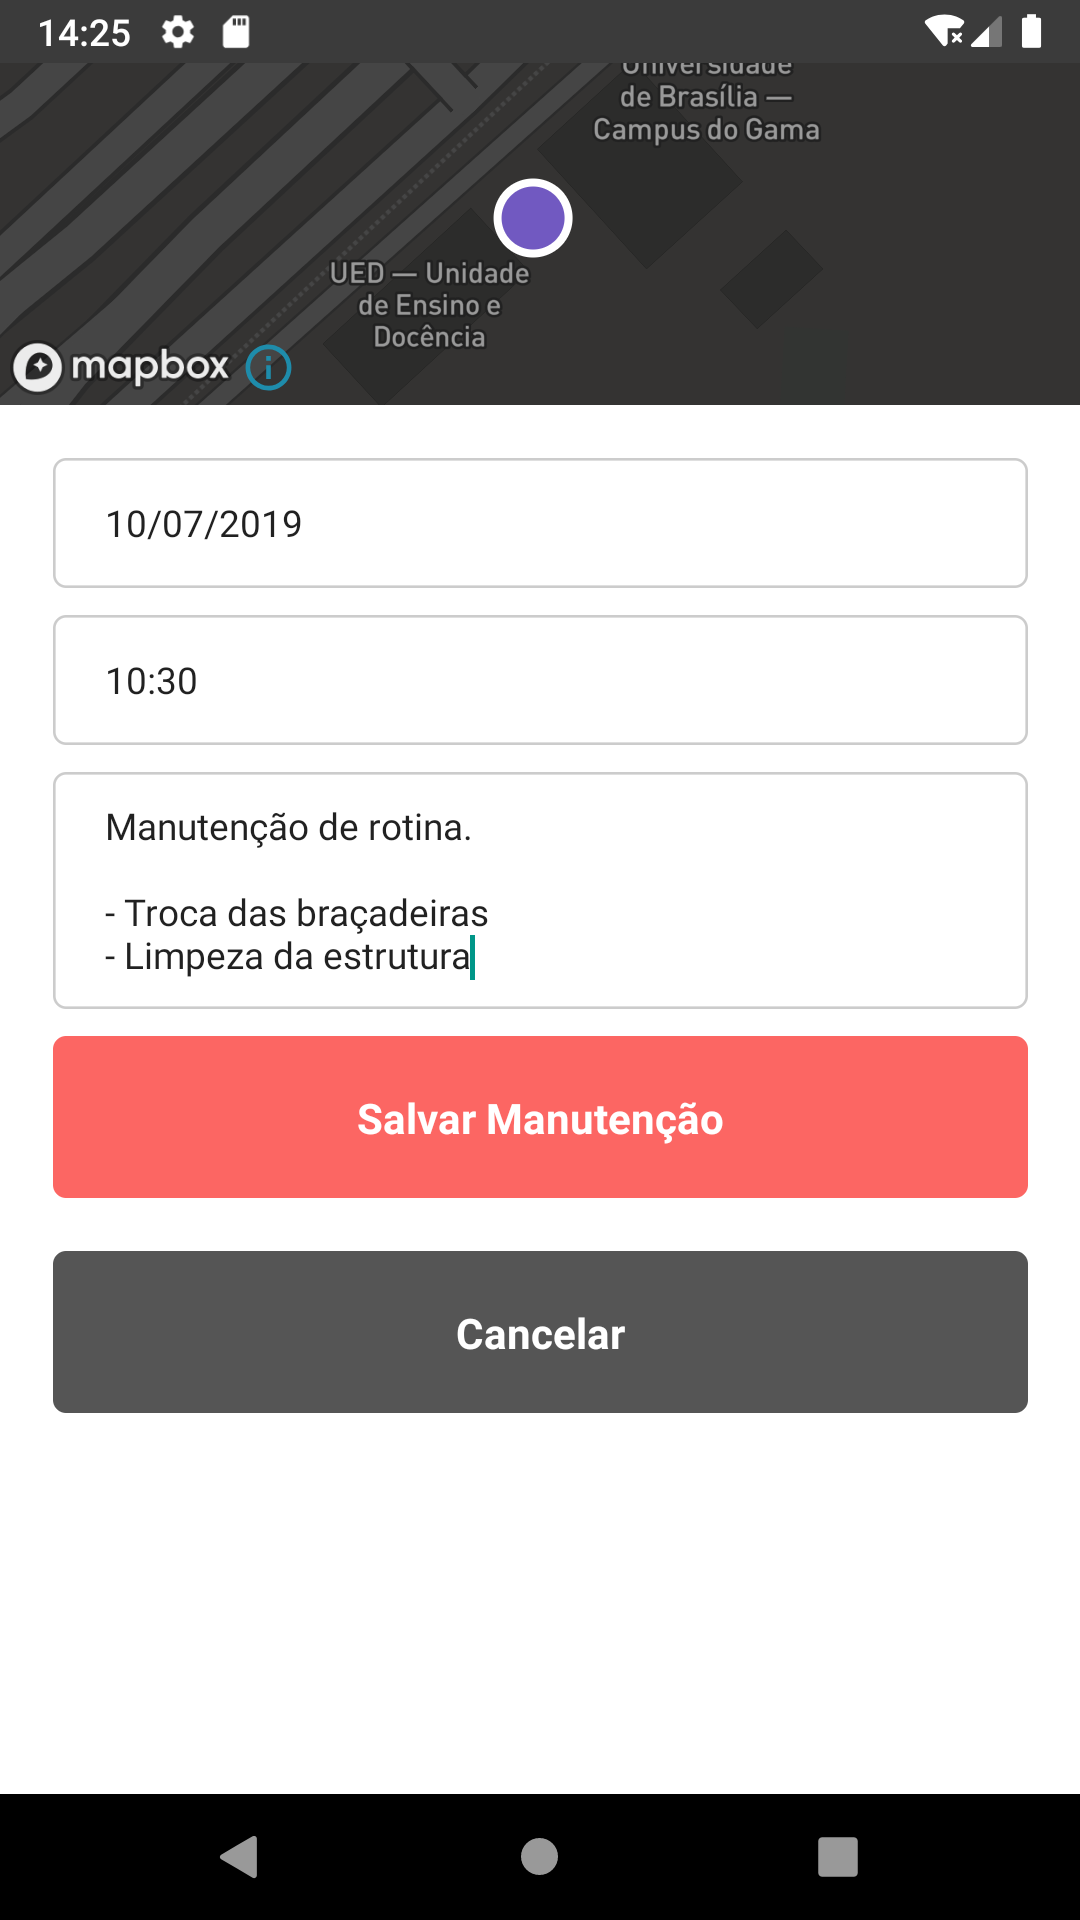
\includegraphics[scale=0.15]{manutencao.png}
        \caption{Tela com as opções de salvar ou cancelar a manutenção.}
        \label{fig:app-manutencao}
    \end{figure}

Assim que a manutenção for salva o aplicativo apresentará um \textit{pop up} informando que o registro foi salvo e indicando o nome do radar o qual o registro pertence, bastando apertar "OK" para fechar a caixa de diálogo, como exemplificado na Figura \ref{fig:app-salvo}.
    
    \begin{figure}[H]
        \centering
        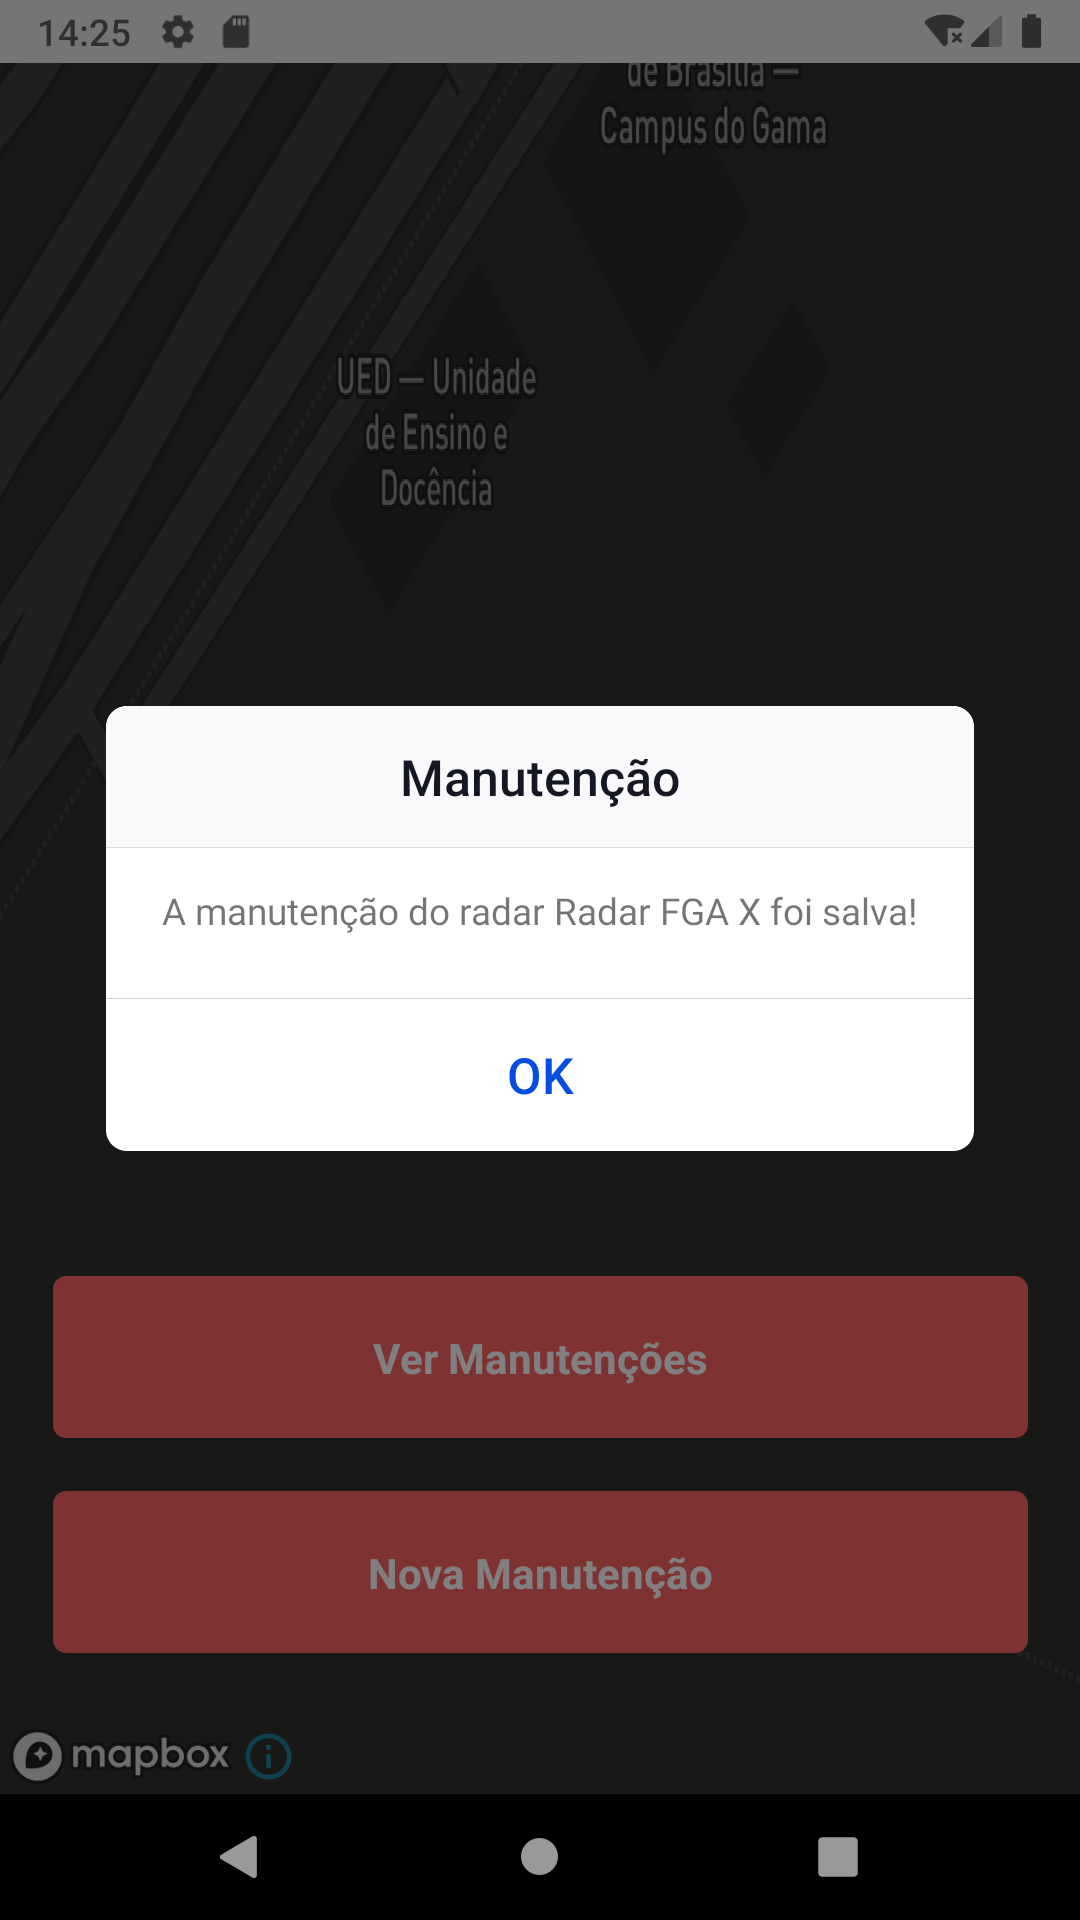
\includegraphics[scale=0.15]{manutencao-salva.png}
\caption{Tela mostrando ao usuário que a manutenção foi salva.}
        \label{fig:app-salvo}
    \end{figure}

Caso o usuário não tenha escolhido nenhuma das opções, mas tenha selecionado o nome do radar na tela principal, o sistema abrirá uma lista com os últimos dez (mais recentes) registros do estado dos componentes do radar selecionado, como mostra a Figura \ref{fig:app-status}. Ao apertar o botar "Fechar" o usuário retorna à tela principal da aplicação.

    \begin{figure}[H]
        \centering
        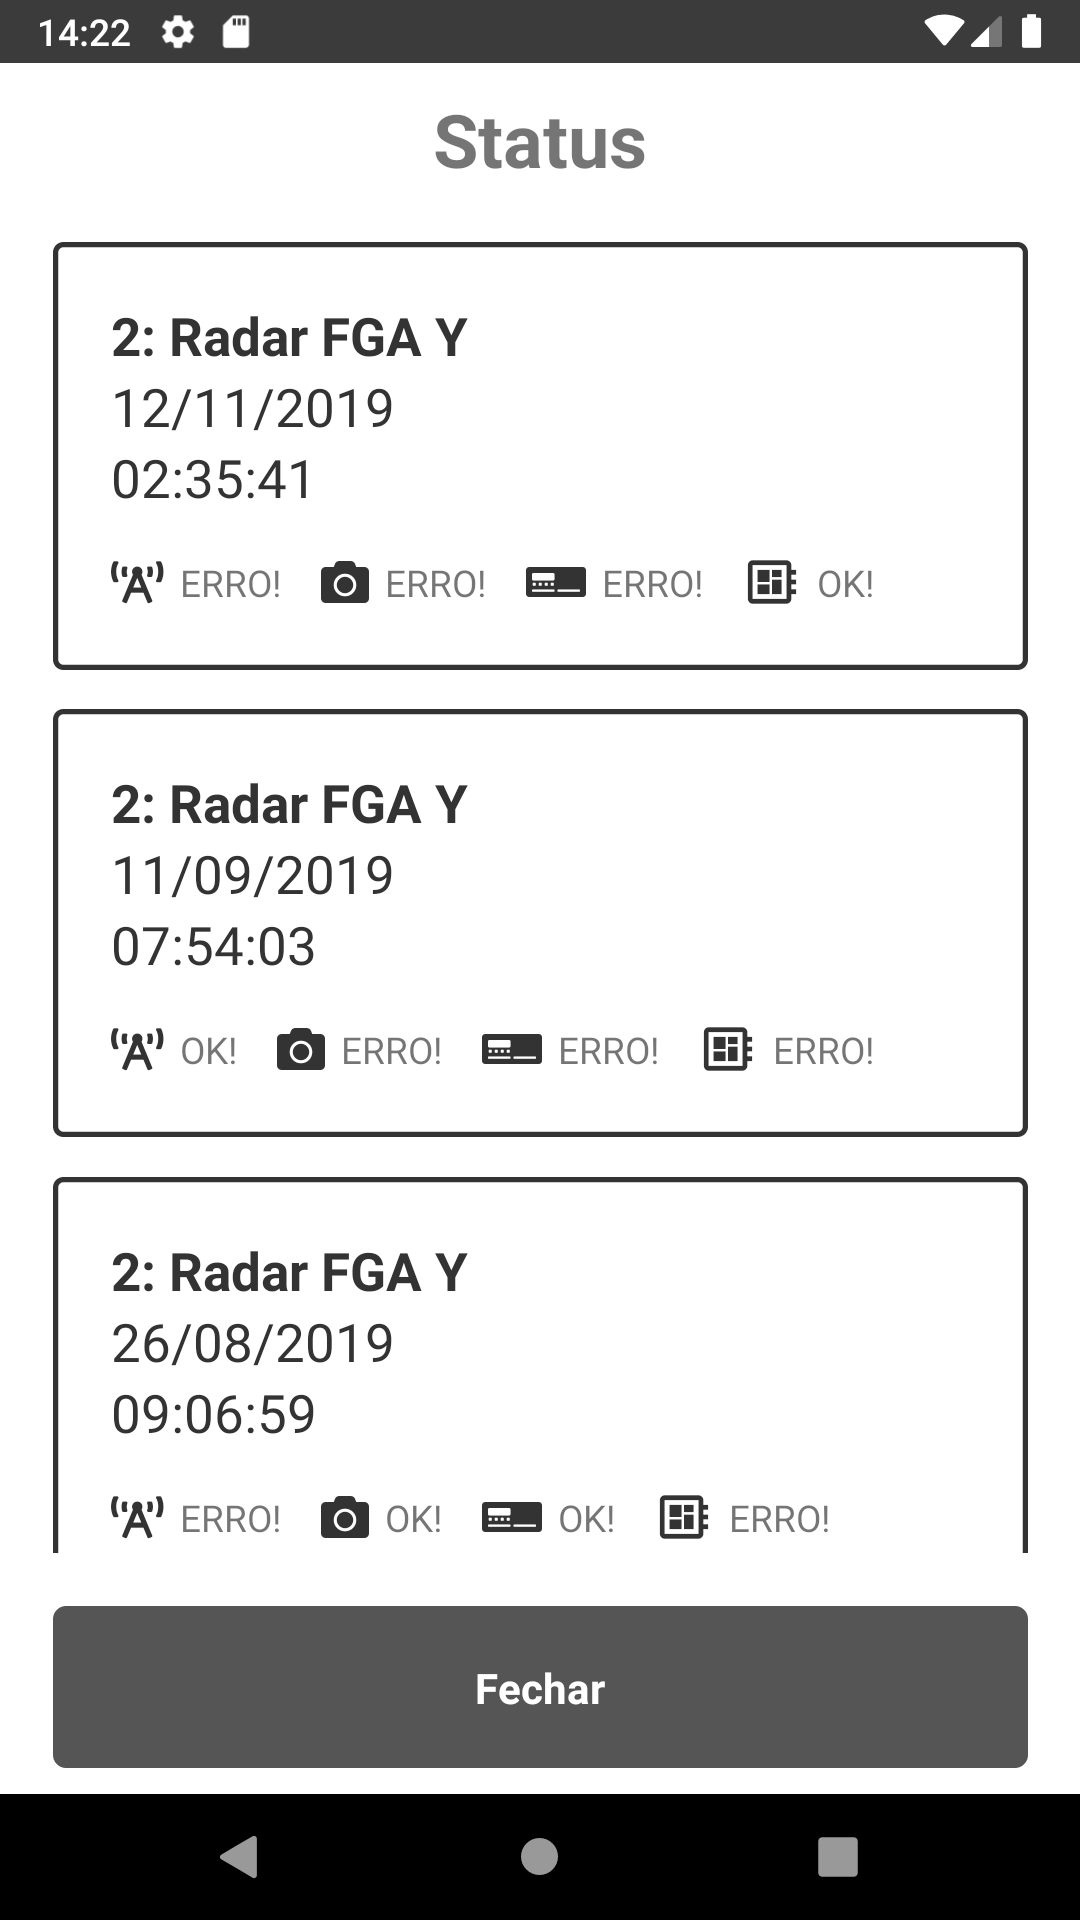
\includegraphics[scale=0.15]{status.png}
        \caption{Tela com os status dos radares.}
        \label{fig:app-status}
    \end{figure}
    
Após feito o uso da aplicação o usuário fica livre para explorar o mapa e registrar operações em outros radares. Caso não seja necessário basta apertar o botão voltar do sistema \textit{android} para fechar a aplicação.
